%Archivo de muestra del informe escrito del curso IE-0499 Proyecto el�ctrico
% utilizando la clase eieproyecto.cls (V.M. Alfaro, febrero de 2013)
%
%pre�mbulo - uso de la clase ``eieproyecto''

%== POR USUARIO (DOCUMENTO FINAL O EN BORRADOR) ---------------------
%usar para el informe final
\documentclass{eieproyecto}

%usar para los informes preliminares (en ``borrador'')
%\documentclass[borrador]{eieproyecto}

%--------------------------------------------------------------------
%inicio del informe
\begin{document}
\frontmatter

%== POR USUARIO (INFORMACION PARA LA PORTADA) -------------------------------
%informaci�n a ser incluida, seg�n corresponda

%t�tulo del proyecto
\title{Soporte de cortado vectorizado en Linux para la cortadora las�r del Arcoslab.}

%nombre completo del autor
\autor{Joshua Torres Morales}

%fecha de la presentaci�n oral
\date{Diciembre 2015}

%tribunal evaluador
%profesor gu�a
\dca{Dr. Federico Alberto Ruiz Ugalde, Ph.D}

%miembros del tribunal (lectores)
\maca{Ing. Sergio Andr�s Valverde Vega}
\mbca{Dr. Leonardo Mar�n Paniagua, Ph.D}

%--------------------------------------------------------------------
%no tocar estas l�neas
\eietitlepage %portada
\cleardoublepage 
\eieaprovalpage %hoja de aprobaci�n
\cleardoublepage

%== POR USUARIO (RESUMEN) -------------------------------------------
%el resumen no debe exceder una p�gina
%Archivo con el texto del resumen
% este no debe exceder una p�gina
\begin{center}\huge{\textbf{Resumen}}\end{center}

%--------------------------------------------------------------------
\noindent

En el presente proyecto se plantea el desarrollo e implementaci�n de programa de aplicaci�n
para la realizaci�n de cortes vectoriales utilizando la cortadora l�ser. "Laser Spectrum H-Series 20x12 5th Gen".

Para el desarrollo de dicha aplicaci�n se plantea un dise�o modular donde diversos sub programas combinados ofrecen distintas funcionalidades, entre ellas se incluyen la extracci�n de informaci�n  gr�fica a partir de un archivo PDF y la interpretaci�n de dicha informaci�n para la generaci�n de comandos de corte que puedan ser utilizados por la cortadora l�ser.

Estos dise�os fueron implementados en el lenguaje de programaci�n Python, donde se utiliz� el paradigma de programaci�n orientada a objetos para lograr la modularidad requerida por el dise�o. 

Finalmente en el documento se presentan diversas pruebas de cortes realizados con el programa desarrollado y se plantean diversas recomendaciones para la el desarrollo futuro de la aplicaci�n. 



  
 
\cleardoublepage

%--------------------------------------------------------------------
%las siguientes son las secciones iniciales del informe (�ndices)
\tableofcontents*  %�ndice general

%los siguientes �ndices pueden omitirse, ponerse en la misma p�gina, o en p�ginas separadas
\clearpage
\listoffigures  %�ndice de figuras

%\clearpage
%\listoftables   %�ndice de cuadros
\cleardoublepage

%== POR USUARIO (NOMENCLATURA) --------------------------------------
%nomenclatura - definir todos los s�mbolos, variables
% y acr�nimos utilizados en el informe
%Lista de la nomenclatura utilizada en el texto
% constantes, variables, s�mbolos, acr�nimos, etc.

\chapter{Nomenclatura}
%--------------------------------------------------------------------

\begin{description}[labelindent=1cm,labelwidth=2.25cm,align=left,leftmargin=3.45cm]  %no cambiar esta l�nea
	\item [ARCOSLAB] Autonomous Robots and Cognitive Systems Laboratory.
	\item [CAD] Computer Assisted Design.	
	\item [CNC] Computer Numerical Control.
	\item [GUI] Graphical User Interfase. 	
	\item [Laser] Light Amplification by Stimulated Emission of Radiation.
	\item [NC] Numerical Control.	
	\item [PCB] Printed Circuit Board.
	\item [PD] 	Porcentaje de potencia de corte deseada. 
	\item [PDF] Portable Data File.
	\item [$P(PD)$] Valor del byte de potencia de corte para los comandos de corte.
	\item [PPI] Pixels per inch.
	\item [PS] Post-Script. 
	\item [WLAN] Wireless Local Area Network.
	\item [X(t)]  Variaci�n de la coordenada X de la curva de B�zier a trav�s en el tiempo.
	\item [$X_0$] Localizaci�n en el eje X del punto inicial de la curva de B�zier.
	\item [$X_1$] Localizaci�n en el eje X del primer  punto de control de curvatura de la curva de B�zier.
	\item [$X_2$] Localizaci�n en el eje X del segundo punto de control de curvatura de la curva de B�zier.
	\item [$X_3$] Localizaci�n en el eje X del punto final de la curva de B�zier.
	\item [Y(t)]  Variaci�n de la coordenada Y de la curva de B�zier a trav�s en el tiempo.
	\item [$Y_0$] Localizaci�n en el eje Y del punto inicial de la curva de B�zier.
	\item [$Y_1$] Localizaci�n en el eje Y del primer  punto de control de curvatura de la curva de B�zier.
	\item [$Y_2$] Localizaci�n en el eje Y del segundo  punto de control de curvatura de la curva de B�zier.
	\item [$Y_3$] Localizaci�n en el eje Y del punto final de la curva de B�zier.
	
\end{description}


%--------------------------------------------------------------------
%no tocar estas l�neas
\mainmatter
\pagestyle{eieheadings}

%== POR USUARIO (CONTENIDO DEL INFORME) -----------------------------
%cap�tulos del trabajo (puede ser un solo archivo o
% separarse los cap�tulos en archivos independientes)
% usar \include{nombre_archivo} para incluir cada cap�tulo

%documento con el cuerpo del informe.
%puede ser un solo archivo o varios, por ejemplo uno por cada cap�tulo
%- cap�tulo ---------------------------------------------------------
\chapter{Introducci�n} \label{sec:L01}
%%%%%%%%%%%%%%%%%%%%%%
%\section{Justificaci�n}

\section{Alcance del proyecto}
El Arcoslab (Autonomous Robots and Cognitive Systems Laboratory) cuenta con una cortadora l�ser "Laser Spectrum H-Series 20x12 5th Gen " , la cortadora cuenta con dos modos de operaci�n: cortado rasterizado y cortado vectorial.
El cortado vectorial es utilizado en el Arcoslab para la confecci�n de PCB (tarjetas de circuito impreso, para los diversos proyectos del laboratorio. El software existente para el control de la cortadora l�ser presenta ciertos inconvenientes: 

\begin{enumerate}
	\item El software es propietario por lo que no puede ser modificado para adecuarse a las necesidades del laboratorio.
	\item El software funciona exclusivamente con el  sistema operativo Microsoft Windows lo que obliga al laboratorio a hacer uso de m�quinas virtuales con este sistema operativo; puesto que las computadoras del laboratorio utilizan la distribuci�n Debian del sistema operativo GNU/Linux.
\end{enumerate}

Por estos motivos en este proyecto se plantea el dise�o y puesta en funcionamiento de un software capaz de realizar las tareas de control necesarias para dar soporte de cortado vectorizado en el sistema operativo Linux a la cortadora l�ser del laboratorio adem�s de generar toda la documentaci�n necesaria para que dicho software pueda ser modificado en el futuro.

\section{Objetivos}

\subsection{Objetivo general}
Dise�ar e implementar un programa de aplicaci�n para el control de la cortadora l�ser "Laser Spectrum H-Series 20x12 5th Gen " del Arcoslab que tome un archivo PDF y lo transforme en comandos de corte.

\subsection{Objetivos espec�ficos}
Para el desarrollo de este proyecto se establecieron los siguientes objetivos:
\begin{itemize} % lista con vi�etas
        \item Investigar y documentar el protocolo de comunicaci�n de la cortadora l�ser.
        \item Dise�ar el software de cortado, un ejecutor de estructuras de datos hacia la cortadora, un parser de PDF a estructura de datos vectoriales, un extractor de datos del PDF y una interfaz gr�fica de usuario.
        \item Realizar la programaci�n e implementaci�n de los programas anteriores.
        \item Realizar pruebas de funcionamiento.
        \item Escribir un manual de instrucciones y un tutorial para los programas desarrollados.
\end{itemize}

\section{Metodolog�a}
El desarrollo del trabajo incluy� los siguientes pasos y procedimientos, listados en secuencia:

\begin{enumerate}  %lista numerada
        \item Investigaci�n bibliogr�fica sobre el principio de funcionamiento de las maquinas CNC, en especial de las cortadoras l�ser y m�quinas de prototipado de PCB.
        \item Investigaci�n bibliogr�fica acerca de los algoritmos, definiciones y est�ndares fijados para la renderizaci�n de archivos PDF, adem�s de terminolog�a general utilizada en Gr�ficos Por Computadora.
        \item Investigaci�n bibliogr�fica sobre el protocolo de comunicaci�n utilizado por la cortadora l�ser Full Spectrum Laser 5th Gen. 
        \item Dise�o de las distintas estructuras de datos y algoritmos necesarios para la elaboraci�n de los de los distintos programas de aplicaci�n.
        \item Dise�o de la interfaz gr�fica de usuario.
        \item Selecci�n de un lenguaje de programaci�n y paradigma de programaci�n adecuados.  
        \item Implementaci�n de los distintos programas de aplicaci�n utilizando el lenguaje de programaci�n seleccionado.   
        \item Elaboraci�n de pruebas de funcionamiento apropiadas, para comprobar el funcionamiento de los programas implementados.
        \item Realizaci�n de Debugging para corregir los errores encontrados luego de realizar las pruebas.
        \item Escritura del manual de usuario y tutorial de uso para los programas desarrollados. 
\end{enumerate}

\section{Contenido}
A continuaci�n se describe la estructura de este documento:

\begin{itemize}
        \item En el Cap�tulo \ref{sec:L01}, se ha descrito a profundidad la justificaci�n del proyecto, el motivo de su desarrollo, los objetivos que �ste debe cumplir, y la metodolog�a seguida para la elaboraci�n de los diversos programas de aplicaci�n.
        \item En el Cap�tulo \ref{sec:L02}, se encuentra una descripci�n de la teor�a b�sica de funcionamiento de las maquinas herramientas que utilizan control CNC, adem�s se incluye una explicaci�n de los diversos conceptos de redes de comunicaciones y gr�ficos por computadora que son utilizados por los distintos programas desarrollados, finalmente se incluye la documentaci�n del protocolo de comunicaci�n de la cortadora l�ser.  
        \item En el Cap�tulo \ref{sec:L03}, se encuentra un an�lisis de los dise�os desarrollados para la creaci�n de los programas de aplicaci�n adem�s se incluye un an�lisis de las consideradas para implementar estos dise�os. 
        \item En el Cap�tulo \ref{sec:L04}, se presentan los resultados obtenidos con los programas desarrollados y se describen las pruebas realizadas a estos programas.
        \item En el Cap�tulo \ref{sec:L05}, se exponen las conclusiones del proyecto y recomendaciones para el desarrollo posterior de los programas dise�ados.
\end{itemize}

%- declaraci�n de un cap�tulo ---------------------------------------

\chapter{Base te�rica} \label{sec:L02}

\section{Teor�a B�sica de Maquinas CNC}

\subsection{Mecanizado}

El mecanizado de un material seg�n \cite{cnc_Basics}  se refiere a la aplicaci�n de uno o varios procesos sobre una materia prima que permita alterar dicha materia de manera controlada hasta alcanzar una forma deseada. Existen dos tipos de alteraci�n que se le puede efectuar a la materia prima, alteraciones sustractivas que consisten en procesos de remoci�n de material mediante cortes, abrasiones o remociones de viruta hasta alcanzar la forma deseada. El segundo tipo de alteraciones que puede ser efectuado se conoce como aditivas, en estos procesos sobre la materia prima se van depositando capas de material hasta alcanzar la forma final deseada.  
Las alteraciones sobre la materia prima se realizan por medio de maquinaria denominada maquinas herramientas. \citep{cnc_Basics}   

El mecanizado se utiliza en procesos industriales de fabricaci�n, en particular para este trabajo es de inter�s el proceso de fresado de las PCB.

Un PCB es una placa de substrato no conductor, que ofrece soporte mec�nico y conecta mediante pistas de material conductor distintos componentes el�ctricos para formar un circuito.

El fresado de las PCB consiste en el proceso de remover �reas de cobre de una placa de circuito impreso para formar las pistas conductoras, generalmente se realiza con una fresadora de ah� su nombre, pero se puede realizar con otras m�quinas herramientas que realicen alteraciones sustractivas, a estas m�quinas herramientas se les conoce con el nombre colectivo de ''PCB prototyper''. \citep{cnc_Basics} 

\subsection{Control Num�rico por Computador (CNC)}
El control num�rico (CN) puede ser definido seg�n \cite{cnc_Handbook} como la operaci�n de m�quinas herramientas por medio de instrucciones espec�ficamente codificas que son enviadas al sistema de control de la m�quina.

Las primeras m�quinas herramientas que utilizaban el control num�rico, necesitaban de un operador que se colocaba  delante de un panel de control, el operador introduc�a las instrucciones necesarias para generar la pieza requerida y controlaba as� la m�quina. \citep{cnc_Handbook} 

Seg�n \cite{cnc_Handbook}, alrededor del a�o de 1972, se introdujo en las empresas de manufactura el concepto de Control Num�rico por Computador (CNC), en el CNC el operador es sustituido por un computador, por lo que no es necesario tener un operador frente al panel de control de la m�quina herramienta, en un sistema CNC moderno el encargado de enviar las instrucciones a la m�quina herramienta es un micro controlador.      

Al conjunto de todas las instrucciones necesarias para crear una pieza especifica, se le conoce como programa CNC, este programa puede ser guardado para ser utilizado en un futuro en la reproduci�n de piezas. \citep{cnc_Handbook} 

En la fabricaci�n de un PCB se requiere primero realizar el dise�o del circuito, luego utilizar un programa de dise�o asistido por computador (CAD) para generar el archivo de layout. El archivo de layout contiene la informaci�n sobre los puntos de conexi�n de los dispositivos electr�nicos, los disipadores de calor y las pistas que deben ser cortadas sobre el substrato.

Una vez obtenido el archivo de layout este es utilizado para generar el programa CNC y as� enviar las instrucciones necesarias a la m�quina herramienta para producir el PCB. \citep{cnc_Handbook}      

\subsection{Cortadora L�ser }
Para \cite{cnc_Handbook} existen diversos tipos de m�quinas herramientas que utilizan el control CNC, entre las que realizan procesos sustractivos podemos mencionar los tornos, fresadoras, cortadoras de plasma, cortadoras l�ser y tambien cortadoras con chorro de agua. 
 
Entre las que realizan procesos aditivos podemos mencionar las impresoras en 3D. 
Para este trabajo el estudio se concentr� en un tipo espec�fico de m�quina herramienta: las cortadoras l�ser y en su uso como un ''PCB prototyper''.

Las cortadoras l�ser utilizan dispositivos �pticos para dirigir la salida de un l�ser de alta potencia hacia el material que va a ser mecanizado vaporiz�ndolo, quem�ndolo o derriti�ndolo. 

Como lo expresa \cite{cnc_Handbook}, el sistema CNC se encarga de dirigir el movimiento del material al ser cortado o del dispositivo �ptico para formar el patr�n de corte requerido mediante 2 o 3 motores de paso, cada uno encargado de producir el movimiento en alguno de los ejes, adem�s de controlar la potencia de salida del l�ser.  

%Stepper Vs Dc
\begin{figure}[!htb]
        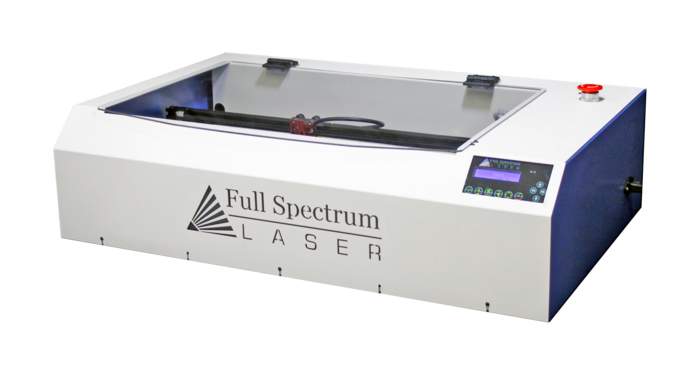
\includegraphics[width=0.7\linewidth]{./Figuras/laser_cutter.png}
        \caption{Cortadora Laser Spectrum H-Series 20x12 tomado de } 
        \label{Stepper}
\end{figure}

\subsection{Motor de paso o Stepper Motor}

Un stepper motor consiste en un motor que al recibir una corriente el�ctrica produce una rotaci�n discreta del eje de transmisi�n del motor, en contra posici�n de un motor DC que produce una rotaci�n contin�a. \citep{stepper}
  
En la figura \ref{Stepper} se muestra la diferencia entre una rotaci�n discreta y una rotaci�n continua.  
%Stepper Vs Dc
\begin{figure}[!htb]
        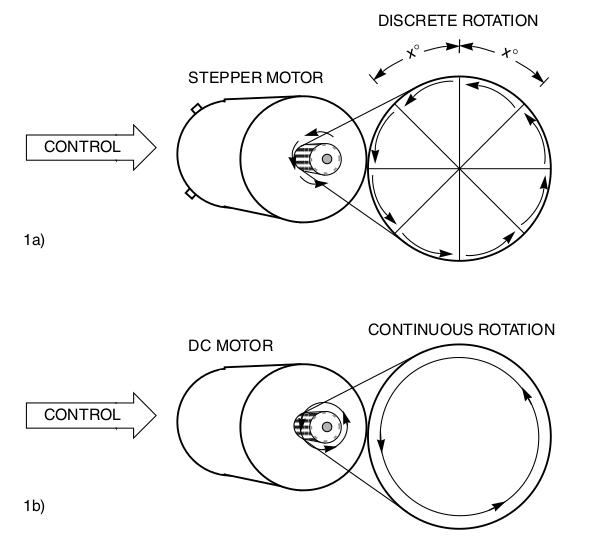
\includegraphics[width=0.7\linewidth]{./Figuras/Stepper.png}
        \caption{Rotaci�n de un motor de paso vs rotaci�n de un motor DC. Tomado de \citep{stepper}} 
        \label{Stepper}
\end{figure}

\subsection{Sistema De Coordenadas Cartesianas}

Como indican los autores \cite{cnc_Basics}, las m�quinas herramientas son usadas para producir dos tipos b�sicos de movimiento, movimientos punto a punto y movimientos de contorno.

En los movimientos punto a punto a la m�quina herramienta se le indica que se dirija a alg�n punto en espec�fico y realice alguna operaci�n, un corte por ejemplo, luego se le pide que se desplace hacia otro punto y realice otra operaci�n y as� sucesivamente hasta terminar el mecanizado de la pieza.

En los movimientos de contorno, la m�quina herramienta produce un solo movimiento continuo que produce la pieza. 
En la figura \ref{Contorno} se muestra un corte realizado con un movimiento de contorno, mientras que en la figura \ref{Punto_punto} se muestra un corte realizado con movimientos punto a punto. Para fresado de las PCB se realizar�n movimientos punto a punto solamente. 

\begin{figure}[!htb]
        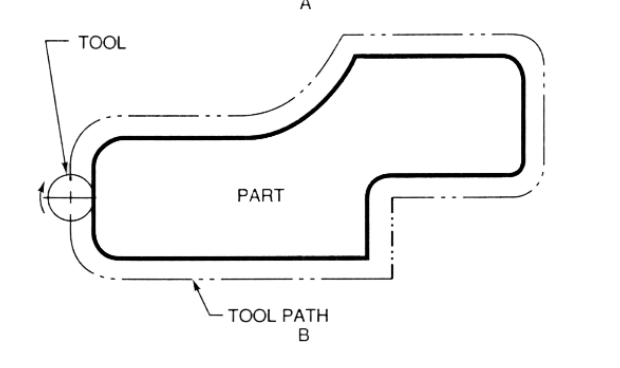
\includegraphics[width=0.7\linewidth]{./Figuras/Contorno_B.png}
        \caption{Corte realizado con un movimiento de contorno. Tomado de \citep{cnc_Basics}} 
        \label{Contorno}
\end{figure}

       
\subsection{Sistemas De Programaci�n}

De acuerdo a \cite{cnc_Basics} para programar los movimientos de una m�quina herramienta por medio de CNC se pueden utilizar dos sistemas de programaci�n distintos denominados sistema absoluto y sistema incremental.
En el sistema incremental, la localizaci�n de los puntos se dan respecto a la distancia y direcci�n del punto anterior, por ejemplo se le puede indicar a la herramienta que debe moverse una pulgada a la derecha del punto anterior.\citep{cnc_Basics}    

La otra alternativa es el sistema absoluto, en este sistema las localizaciones de todos los puntos se dan con respecto a un punto de origen. El punto de origen o punto cero de la m�quina herramienta puede ser seleccionado a conveniencia y generalmente representa la posici�n inicial de la m�quina.
Si se va a utilizar el sistema cartesiano de coordenadas para localizar los puntos programados, el punto cero de la maquina es tomado como el punto cero de las coordenadas cartesianas. \citep{cnc_Basics}

\subsection{Interpolaci�n}
De acuerdo a \cite{oppenheim1998}, la interpolaci�n es un procedimiento para aproximar una funci�n continua a partir de una cantidad discreta de datos conocidos. En el contexto de las m�quinas herramientas, un algoritmo de interpolaci�n le indica al sistema CNC como moverse de un punto a otro. 

Como lo indican \cite{cnc_Basics} existen 5 tipos de algoritmos de interpolaci�n utilizados en las maquinas herramientas: lineal, circular, parab�lica, cubica y espiral.
 
Las interpolaciones parab�lica y cubica son solo utilizadas en industrias que manufacturan piezas de formas muy complejas como la industria aeroespacial y la interpolaci�n espiral es utilizada en m�quinas herramientas que requirieren formar agujeros para tornillos, como por ejemplo los taladros, por este motivo el estudio se concentr� en la interpolaci�n lineal y la interpolaci�n circular solamente.\citep{cnc_Basics}   

\subsubsection{Interpolacion Lineal}
Seg�n \cite{matlab_moler} un algoritmo de interpolaci�n lineal consiste en un procedimiento para encontrar  varias l�neas rectas que unan los puntos programados. Esto es posible por el hecho que dos puntos distintos en un plano permiten determinar un polinomio de primer grado cuyo gr�fico forma una l�nea recta que contiene esos dos puntos.

De acurdo \cite{cnc_Basics} la interpolaci�n lineal requiere solamente de dos puntos programados, el punto de inicio y el punto final, el algoritmo generar� las instrucciones necesarias para que la herramienta produzca un corte en l�nea recta que una estos dos puntos. Estos puntos deben estar en el sistema de coordenadas y el sistema de programaci�n elegidos.

La figura \ref{Interpolacion Lineal} ilustra el resultado de aplicar un algoritmo de interpolaci�n lineal.  
\begin{figure}[!htb]
        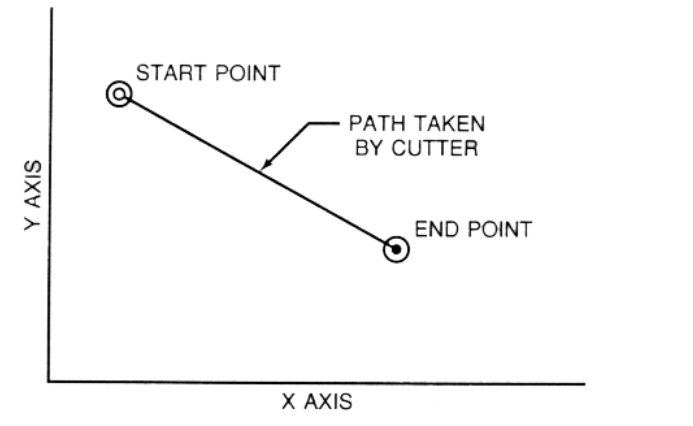
\includegraphics[width=0.7\linewidth]{./Figuras/Interpolacion_Lineal}
        \caption{Ejemplo de un camino recorrido por una cortadora utilizando interpolaci�n Lineal. Tomado de \citep{cnc_Basics}} 
        \label{Interpolacion Lineal}
\end{figure}

Para realizar un patr�n de corte complejo, el punto final del corte anterior se transforma en el punto inicial para el siguiente corte, se procede as� sucesivamente hasta lograr el patr�n requerido.      
Es posible producir curvas utilizando un algoritmo de interpolaci�n lineal, para ello se requiere dividir la curva en segmentos de recta suficientemente cortos. \citep{cnc_Basics}

En la figura \ref{Punto_punto} se muestra un patr�n de corte realizado mediante interpolaci�n lineal. 
\begin{figure}[!htb]
        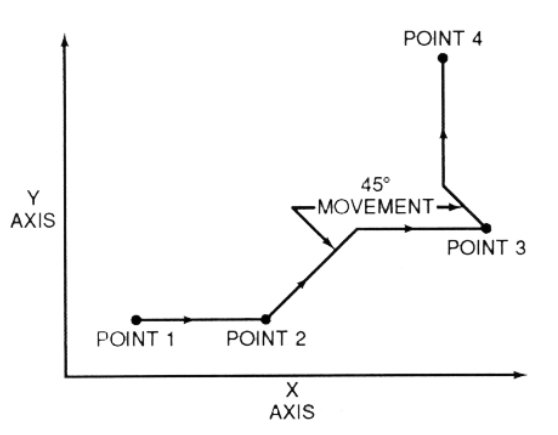
\includegraphics[width=0.7\linewidth]{./Figuras/Punto_punto}
        \caption{Ejemplo de un patr�n de corte de varios puntos programados utilizando interpolaci�n lineal. Tomado de \citep{cnc_Basics}} 
        \label{Punto_punto}
\end{figure}

\subsubsection{Interpolacion Circular}
Continuando con \cite {cnc_Basics}, un algoritmo de interpolaci�n circular consiste en unir los puntos programados mediante un arcos o c�rculos, para lograrlo se necesitan un punto de inicio, un punto final, un punto que localice el centro del c�rculo, el radio del circulo y si el corte se realizar� en sentido de las manecillas del reloj o contrario a estas.   

En la figura \ref{Interpolacion Circular} se muestra un corte realizado por medio de interpolaci�n circular. 

%Stepper Vs Dc
\begin{figure}[!htb]
        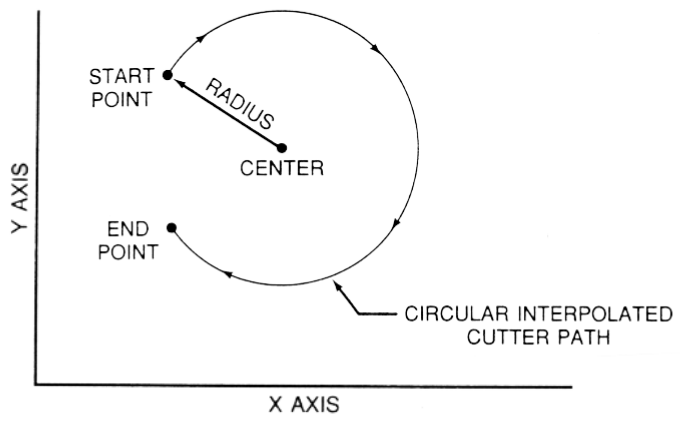
\includegraphics[width=0.7\linewidth]{./Figuras/Interpolacion_Circular}
        \caption{Ejemplo de un camino recorrido por una cortadora utilizando interpolaci�n circular. } 
        \label{Interpolacion Circular}
\end{figure}

\subsection{Estructura Del Programa CNC }

A continuaci�n se discutir� la estructura que tienen los programas CNC utilizados por la cortadora l�ser as� como los comandos con los que dispone el algoritmo de interpolaci�n para realizar los cortes.

De acuerdo a \cite{Alex}, el programa CNC utilizado por la cortadora l�ser "Laser Spectrum H-Series 20x12 5th Gen " est� formado por dos partes: el Header y los comandos de corte.

El header representa informaci�n necesaria para la configuraci�n de la cortadora, tiene un tama�o de 1024 bytes y cuenta con las siguientes partes \citep{Alex}

\begin{enumerate}
        \item 1 byte que define el tipo de corte que se realizar�, para el corte vectorial su valor es de 0x02.  
        \item 135 bytes con un valor de 0x00. 
        \item Un string hexadecimal con los valores 05 00 00 00 00 00 00 00 00 00 00 00 00 00 00 00 00 00 00 00. 
        \item Una estructura de datos llamada Gstruct2 que contiene los par�metros de configuraci�n. 
        \item Un string hexadecimal con los valores 17 00 00 00 00 00 00 00 00 00 00 00 00 00 00 00 00 00 00 00.
        \item Y finalmente 510 bytes con un valor de 0x00.
\end{enumerate}
  
En la figura \ref{Gstruct2} se observa la estructura de Gstruct2, los valores para estos bytes ser�n generados mediante la librer�a libre libjob desarrollada por \cite{Alex} por lo que el estudio se concentrar� en los comandos de corte.  

\begin{figure}[!htb]
        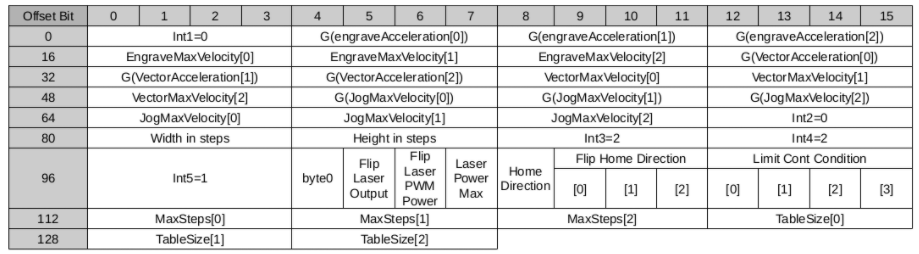
\includegraphics[width=150mm,height=50mm]{./Figuras/Gstruct2.png}
        \caption{Estructura de datos Gstruct2. Tomado de \citep{Alex}. } 
        \label{Gstruct2}
\end{figure}

\subsubsection{Comandos de Corte}

Seg�n \cite{Alex}, para realizar los cortes, la cortadora l�ser cuenta con 4 comandos b�sicos: movimiento en el eje X, movimiento en el eje Y, movimiento en ambos ejes y No Operation.  
Cada comando est� formado por 4 bytes, el primer byte representa el signo del movimiento que se va a realizar, el segundo byte representa la cantidad de steps que se realizaran en el eje X, el tercer byte representa la cantidad de steps que se realizan en el Y y el �ltimo byte representa la potencia utilizada  por el l�ser. En la figura \ref{Cortes} se aprecia la estructura de los comandos de la cortadora.

\begin{figure}[!htb]
        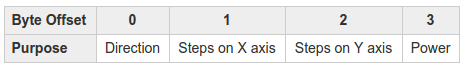
\includegraphics[width=0.7\linewidth]{./Figuras/ComandosDeCorte.png}
        \caption{Estructura de los comandos de corte. Tomado de \citep{Alex}.} 
        \label{Cortes}
\end{figure}

El byte de signo define el sentido de rotaci�n de los motores de paso a paso y funciona de la siguiente manera: El primer bit del primer byte representa el signo del movimiento del eje X el cual toma un valor de cero cuando los movimientos se realizan en la direcci�n positiva y de 1 cuando se realizan en la posici�n negativa, el bit n�mero dos representa el signo del movimiento en el eje Y y funciona de manera an�loga al primer bit.
Si el cabezal de la cortadora se mueve hacia la derecha, los movimientos se consideran movimientos positivos en el eje X, y si se mueve hacia atr�s se consideran movimientos positivos en el eje Y. De forma an�loga si el cabezal de la cortadora se mueve hacia la izquierda o hacia adelante los movimientos se consideran negativos en el eje X y el eje Y respectivamente.      

Los siguientes dos bytes representan la cantidad de steps que deben moverse los motores de paso a paso, para realizar movimientos en el eje X, el segundo byte debe tomar un valor distinto de cero y el tercero un valor de cero. Para realizar movimientos en el eje Y el tercer byte debe tomar un valor distinto de cero y el segundo byte un valor de cero. Finalmente si ambos bytes toman un valor de cero se realizan movimientos simult�neos en ambos ejes.

El �ltimo byte representa la potencia del l�ser que ser� utilizada para realizar el corte, el cual var�a entre cero y cien por ciento. Si el valor de la potencia es de cero por ciento, la cortadora mover� el cabezal siguiendo la trayectoria programada sin realizar ning�n corte en el material. \citep{Alex}

El valor del cuarto byte se calcula con la ecuaci�n \ref{Eq:Power} redondeada al entero m�s pr�ximo y representada en valor hexadecimal. 

\begin{equation}
        \label{Eq:Power}
        P(PD) = PD * \dfrac{255}{100} 
\end{equation}

\section{Gr�ficos Por Computadora}

Los gr�ficos por computadora, seg�n \cite{foley_graphics_c} se refiere a la ciencia de comunicar informaci�n visual por medio de una computadora, es un campo multidisciplinario que utiliza el modelado f�sico y matem�tico para describir formas y figuras.

Entre sus enfoques se encuentran la comunicaci�n entre computadoras y humanos mediante dispositivos tales como monitores, teclados, ratones e impresoras y la comunicaci�n de la computadora con el mundo exterior mediante c�maras. \citep{foley_graphics_c} 

En el contexto de este trabajo, el estudio se centr� en dos conceptos utilizados para la representaci�n de im�genes por computadora. Los gr�ficos vectoriales y los gr�ficos rasterizados.  

\subsection{Gr�ficos Vectoriales}
Indica \cite{foley_graphics_c} que un gr�fico vectorial, es un tipo de gr�fico en el que se utilizan primitivas geom�tricas (puntos, l�neas, curvas o pol�gonos) para representar las im�genes.

En los gr�ficos por computadoras se utilizan los modelos matem�ticos de dichas primitivas para formar el gr�fico. 
Los gr�ficos vectoriales est�n basados en el concepto de vectores, a lo largo del gr�fico se cuentan con puntos de control con una posici�n absoluta en los ejes cartesianos XY, el vector contiene la informaci�n necesaria para unir los puntos de control  mediante las primitivas geom�tricas adecuadas, por ejemplo si se desea trazar una l�nea recta entre dos puntos de control, el vector contendr�a cu�l de los puntos de control se tomar�a como el punto inicial de la recta y cu�l de los puntos de control se tomar�a como el punto final de la recta. Con esta informaci�n es posible calcular la ecuaci�n de la recta que une ambos puntos.      

Adem�s, contiene informaci�n acerca del color, grosor y relleno necesario para realizar el trazado de las primitivas.
Para formar el gr�fico, varios vectores son unidos uno tras otro formando un camino, a este camino se le da el nombre de Path. \citep{foley_graphics_c}

En la figura \ref{bitmap}, se muestran un gr�fico ideal y sus representaciones como un gr�fico vectorial y como un gr�fico raterizado.

\begin{figure}[!htb]
        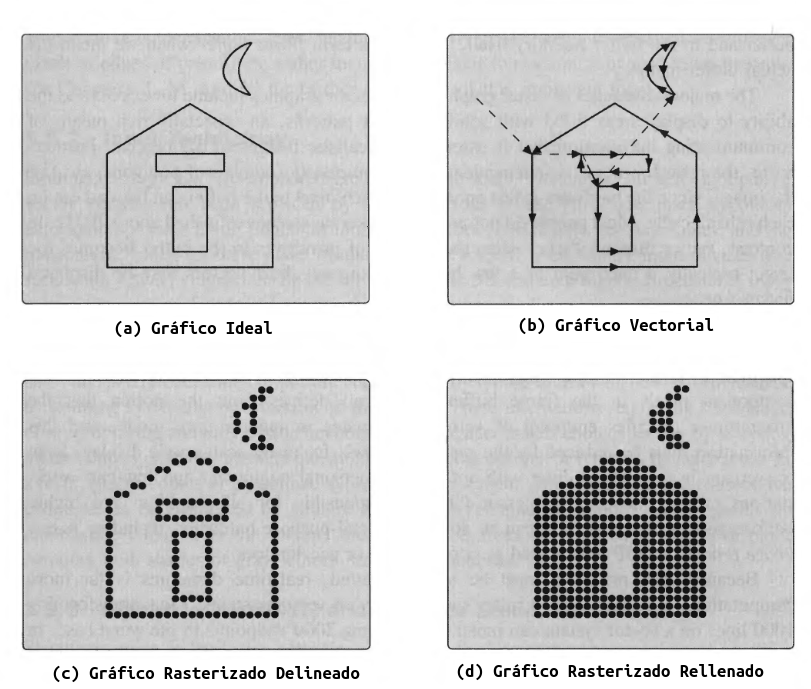
\includegraphics[width=0.7\linewidth]{./Figuras/Graficos_dif.png}
        \caption{Diferencia entre un Gr�fico Ideal, un gr�fico vectorial y un gr�fico raterizado. Tomado de \citep{foley_graphics_c}.} 
        \label{Graficos_dif}
\end{figure}

\subsection{Gr�ficos Rasterizados}

Un gr�fico rasterizado, utiliza una matriz de puntos para representar una grilla rectangular de puntos de color. Cada punto en la matriz representa un punto en el plano cartesiano del monitor, papel, o dispositivo de visualizaci�n, cada punto se representa en la matriz por uno o m�s bits que contienen la informaci�n de color que debe ser desplegada. Por ejemplo en una escala monocrom�tica (de un solo color) cada punto se representa por un solo bit de color, si el bit est� en cero el punto debe ser desplegado en color blanco en el display, mientras que si el bit est� en uno, el punto debe desplegarse en color negro. Un ejemplo de este tipo de gr�fico se muestra en la figura \ref{bitmap}.\citep{foley_graphics_c}     

\begin{figure}[!htb]
        
\includegraphics[width=0.5\linewidth]{./Figuras/bitmap}
        \caption{Gr�fico Rasterizado en escala monocrom�tica. Tomado de \citep{foley_graphics_c}.} 
        \label{bitmap}
\end{figure}
\subsection{Portable Document Format (PDF)}

De acuerdo a \cite{adobe2005pdf} el formato de documento port�til (PDF) es un formato que permite a los usuarios desplegar documentos independientemente del entorno donde fueron creados. 

El formato PDF utiliza el lenguaje de programaci�n PostScript(PS) para describir textos y gr�ficos pero agrega estructuras de control adicionales que permite una descripci�n m�s estructurada que la obtenida utilizando solamente un programa escrito en PS.  

Un documento PDF consiste en una colecci�n de objetos que en conjunto, describen la apariencia de una o m�s p�ginas. Cada p�gina de documento puede contener texto, gr�ficos e im�genes. 

El programa de aplicaci�n que produce el archivo PDF debe generar una descripci�n de la p�gina independiente del dispositivo donde ser� visualizada utilizando la sintaxis del lenguaje de descripci�n.

Un programa que controla un dispositivo de salida espec�fico, por ejemplo un monitor, debe interpretar esta descripci�n y mostrarla en ese dispositivo.

El modelo de imagen de Adobe utilizado en los archivos PDF consiste en una vista bidimensional de los gr�ficos. En esta vista, "pintura" es colocada para representar formas geom�tricas, l�neas o im�genes digitalizadas.
Esta pintura puede ser de varios colores, blanca, negra o en escala de grises.

Para formar los gr�ficos, el contenido es descrito mediante operadores y operandos. \citep{adobe2005pdf}   
    
Seg�n \cite{adobe2005pdf}, para desplegar un archivo PDF es necesario seguir los siguientes pasos:
\begin{itemize}
        \item Extraer los contenidos de cada p�gina, cada stream de contenido es esencialmente un script de PostScript usando procedimientos muy espec�ficos como m para moveto y l para lineto.
        \item Decodificar los textos o gr�ficos comprimidos utilizando el filtro apropiado.
        \item Poner la informaci�n en el orden correcto
        \item Transmitir el programa en PostScript hacia el dispositivo de salida.
\end{itemize}

\subsection{Sintaxis de un archivo PDF}

Los archivos PDF usan estructuras de datos llamadas Objetos, estos pueden ser de 8 tipos, seg�n lo expresa \cite{adobe2005pdf}:

\begin{itemize}
        \item Valores booleanos.
        \item N�meros reales o n�meros enteros
        \item Cadenas de caracteres (Strings)
        \item Nombres
        \item Arreglos de datos (Arrays)
        \item Diccionarios
        \item Flujos de datos (streams)
        \item Objetos de tipo nulo.
\end{itemize}
 
Los objetos pueden usar etiquetas para que otros objetos se refieran a ellos, un objeto con una etiqueta se llama un objeto indirecto. 

La etiqueta usada para referirse a los objetos indirectos consiste en dos partes: Un n�mero entero llamado n�mero de identificaci�n que generalmente va en orden secuencial seg�n su orden de creaci�n, as� por ejemplo el primer objeto creado tendr�a n�mero de identificaci�n 01, y el siguiente objeto creado tendr�a como n�mero de identificaci�n 02 y as� sucesivamente. Sin embargo la numeraci�n se puede realizar de forma arbitraria mientras cada objeto se le asigne 
un n�mero �nico y un n�mero no negativo llamado n�mero de generaci�n, la primera vez que un objeto es creado se le asigna un n�mero de generaci�n de cero. Si el archivo PDF es modificado posteriormente por alg�n programa, el n�mero de generaci�n puede tomar un valor distinto de cero que representa cuantas veces se ha modificado el objeto. \citep {adobe2005pdf}

A continuaci�n se observa la sintaxis de un objeto reci�n creado.

\begin{lstlisting}[language=PostScript, caption=Ejemplo de Un Objeto Indirecto en PDF] 
        17 0 obj
           ...
    endobj
\end{lstlisting}

En el contexto de los gr�ficos vectoriales los objetos de inter�s son los objetos tipo stream.
 
\subsubsection{Objetos de Flujo de Datos}

Los objetos tipo stream, \cite{adobe2005pdf}, son objetos que contienen secuencias de bytes que pueden alcanzar cualquier tama�o requerido, esta secuencia de bytes se encuentra antecedida por la palabra clave stream y precedida por la palabra clave endstream.

Cada stream cuenta con una entrada que representa el tama�o del stream en bytes. Ademas pueden contar una entrada adicional llamada filtro de compresi�n. Si esta entrada est� presente, el stream de datos ha sido comprimido utilizando el algoritmo Flate-Deflate. \citep{adobe2005pdf}

\begin{minipage}{\linewidth}    
        \begin{lstlisting}[language=HTML, caption=Ejemplo de un Stream Binario Codificado] 
        3 0 obj
                << /Length 4 0 R 
                   /Filter /FlateDecode >>
                
                stream
                        4E 6F 76 20 73 68 6D 6F 7A 20 6B 61 20 70 6F 70 2E 06 79
                endstream
        endobj
    \end{lstlisting}
\end{minipage}

\subsubsection{Algoritmo Flate-Deflate}

El algoritmo de compresi�n Flate para \cite{adobe2005pdf} es utilizado cuando se requiere comprimir informaci�n que forma secuencias, como los archivos de texto. Este algoritmo realiza una compresi�n libre de p�rdidas.
  
Para descomprimir los archivos comprimidos con el algoritmo Flate, se utiliza el algoritmo Deflate. Ambos algoritmos est�n implementados en la librer�a ZLIB la cual ha sido portada a varios lenguajes de programaci�n. \citep{adobe2005pdf}  
 
\subsection{Post-script}
PS es un lenguaje de computadoras utilizado para la creaci�n de gr�ficos vectoriales. 
Un gr�fico vectorial en PDF est� formada por varios operandos y operadores en PS que son guardados en un objeto tipo Stream y pueden o no ser comprimidos usando el filtro "Flate Decode"\citep{adobe2005pdf}

\subsection{Operadores PS para Gr�ficos Vectoriales}
Los caminos (Paths) son estructuras de datos que definen formas, trayectorias y regiones en una imagen en PS, el camino est� compuesto por segmentos que pueden ser l�neas rectas, curvas, etc. conectadas o no unas con otras.  Un par de segmentos est�n conectados entre s� solo si estos est�n definidos de forma consecutiva, con el segundo segmento del camino iniciando justo donde termina el primero.   

Los objetos gr�ficos son definidos por una secuencia de operadores utilizados para construir un camino. 

La descripci�n de una p�gina inicia con un camino vaci�, los operadores de construcci�n son agregados de manera secuencial iniciando ya sea con un operando Moveto o un operando Rect�ngulo.

Al camino en construcci�n se le conoce como  camino actual o Current Path y al punto final del segmento agregado m�s recientemente al camino actual, se le conoce como punto actual o Current Point. \cite{adobe2005pdf}

A continuaci�n se presentan los operadores utilizados en PS para gr�ficos vectoriales:

\subsection{Moveto}
Sintaxis: X Y m
El operador moveto comienza un nuevo path moviendo el Current Point hacia las coordenadas [X,Y].   

\subsection{Lineto}
Sintaxis: X Y l
El operador lineto agrega una l�nea recta al camino, la l�nea recta inicia en el Current Point y termina en las coordenadas [X,Y]. El nuevo Current Point es el punto [X,Y].

\subsection{Curveto}
Sintaxis: $X_1$  $Y_1$ $ X_2$  $Y_2$  $X_3$  $Y_3$ c
El operador curveto agrega una curva cubica de B�zier al camino, la curva inicia en el Current Point y termina en las coordenadas [$X_3$,$Y_3$]. La curva de B�zier utiliza los puntos [$X_1$,$Y_1$] y [$ X_2$,$Y_2$] como puntos de control. El nuevo Current Point es el punto [$X_3$,$Y_3$]. \citep{adobe2005pdf}
  
\subsubsection{Curvas Cubicas De B�zier}
Una curva de B�zier, \cite{adobe2005pdf}, es un modelo matem�tico utilizado para representar curvas indefinidamente 
escalables.

El modelo consiste en curvas param�tricas con la forma de un polinomio de Bernstein de grado N, una curva c�bica de B�zier utiliza entonces, un polinomio de Bernstein de grado 3. En las ecuaciones \ref{Eq:Bezier1} y \ref{Eq:Bezier2} se muestra la parametrizaci�n para una curva c�bica de B�zier en las coordenadas XY.
  
Las curvas cubicas de B�zier utilizan cuatro puntos para controlar la forma de la curva: 

\begin{enumerate}
	\item El punto donde inicia la curva [$X_0$,$Y_0$]
	\item Un primer punto de control [$X1$,$Y1$]
	\item Un segundo punto de control [$X2$,$Y2$]
	\item El punto donde finaliza la curva [$X_3$,$Y_3$]
\end{enumerate}

Para valores del par�metro $t$ en el intervalo [$0.0$,$1.0$], se obtienen puntos contenidos en la curva entre los puntos [$X_0$,$Y_0$] y [$X_3$,$Y_3$] utlizando las ecuaciones \ref{Eq:Bezier1} y \ref{Eq:Bezier2}.  \citep{adobe2005pdf}

\begin{equation}
        \label{Eq:Bezier1}
        X(t) = (1 - t)*X_0 + 3t*(1 - t)*X_1 + 3t*(1 - t)*X_2 + t*X_3
\end{equation}

\begin{equation}
        \label{Eq:Bezier2}
        Y(t) = (1 - t)*Y_0 + 3t*(1 - t)*Y_1 + 3t*(1 - t)*Y_2 + t*Y_3
\end{equation}

\subsection{Rectangle}
Sintaxis: X Y Ancho Altura re
El operador rectangle agrega un rect�ngulo al camino, la esquina inferior izquierda del rect�ngulo se ubica en las coordenadas [X,Y] el rect�ngulo tiene un tama�o dado por los operandos Ancho y Altura.   

\subsection{Closepath}
Sintaxis: h
El operador Closepath cierra el camino agregando una linea recta desde el "Current Point" hasta el punto inicial del primer segmento en el "Current Path". \cite{adobe2005pdf}

%\section{Abstract Data structures}
%Queue:
%Stack:

\section{Redes de Comunicaciones}

\subsection{Modelo de Referencia TCP/IP }
Seg�n indica \cite{tanenbaum2011Redes}, en redes de computadoras, la suite TCP/IP es un conjunto de protocolos de comunicaci�n utilizado en internet y otras redes similares que provee de un modelo de referencia de como una comunicaci�n end-to-end debe transmitir, empacar, enrutar y direccionar la informaci�n.   
Esta funcionalidad est� organizada en cuatro capaz de abstracci�n, para prop�sitos de realizar la conexi�n entre la cortadora l�ser y la computadora encargada de enviar el programa CNC, el estudio se centrar� en 3 de las capas del modelo: la capa de interred, la capa de transporte y la capa de aplicaci�n.    

\subsection{La Capa de Interred � IP}
La Capa de Interred tambi�n conocida como protocolo de Internet (IP), es un protocolo de comunicaci�n que permite la comunicaci�n entre un dispositivo emisor y un dispositivo receptor conocido por el nombre de Host, el objetivo de esta capa es que cada Host pueda enviar paquetes de informaci�n el uno al otro a trav�s de una red de comunicaciones, para ello cada Host cuenta con una direcci�n que los distingue de los dem�s miembros de la red llamada direcci�n IP.  
 
La direcci�n IP es un n�mero de 32 bits (versi�n 4 del protocolo) o de 128 bits (versi�n 6 del protocolo), las direcciones IP son utilizadas por los enrutadores para saber a d�nde enviar cada paquete que circula la red. \citep{tanenbaum2011Redes}   

\subsection{La Capa de Transporte � TCP}

\cite{tanenbaum2011Redes} indica que la Capa de Transporte tambi�n llamada protocolo de control de transmisi�n (TCP) es un protocolo de comunicaci�n que funciona como una capa de abstracci�n extra que se coloca por encima del protocolo IP, esta capa fue dise�ada para permitir que varios Host se puedan comunicar entre ellos de una forma confiable y sin errores.       

El protocolo TCP presenta una capa de abstracci�n a la aplicaci�n que utiliza la suite TCP/IP , de esta forma la aplicaci�n no necesita saber c�mo se realizan las transacciones en el protocolo IP sino que desde el punto de vista de la aplicaci�n, esta se est� comunicando mediante una comunicaci�n punto a punto directamente con el otro Host por medio de un socket de comunicaci�n. 

Un socket de comunicaci�n TCP es una representaci�n abstracta de la conexi�n punto a punto entre dos Host, el socket requiere de una direcci�n IP y un n�mero de puerto para ambos Host y de esta forma le presenta a la aplicaci�n una forma de comunicarse con otro Host. Los puertos permiten que entre los dos Host existan varios canales de comunicaci�n simult�neos, desde el punto de vista de la aplicaci�n es como si ambos Host estuvieran conectados mediante varios cables. \citep{tanenbaum2011Redes}   
 
\subsection{Protocolo de Comunicaci�n De La Cortadora L�ser} \label{sec:L2.3.4}

Finalmente para establecer la comunicaci�n entre la computadora y la cortadora l�ser es necesario un protocolo de comunicaci�n que se sit�a por encima del protocolo TCP, este protocolo representa la capa de aplicaci�n de la suite TCP/IP.

Las comunicaciones con la cortadora se realizar�n por medio del programa de cortado desarrollado. Tanto la computadora que env�a el programa CNC, como la cortadora l�ser estar�n conectadas a una misma red inal�mbrica local (WLAN) y los mensajes enviados y recibidos desde y hacia la cortadora estar�n en formato ASCII. 

A continuaci�n se presentaran los pasos necesarios para establecer la comunicaci�n entre la cortadora l�ser y la computadora para ello se cita a \cite{Alex}:

\begin{enumerate}
        \item El primer paso para establecer la comunicaci�n es crear un Socket TCP y conectarlo al puerto de comunicaci�n 12345 de la cortadora l�ser, denominado iTalk por el fabricante. Adicionalmente se requiere crear un Socket y conectarlo con el puerto 12346 de la cortadora para el env�o del programa CNC.
        \item Si la conexi�n fue exitosa,se iniciara una sesi�n de comunicaci�n y la cortadora responder� con el mensaje " 100 Hello 192.168.16.143. FSL Laser Ready, your session ID 00000001\textbackslash n"
        \item Luego se env�a el mensaje "xjob\textbackslash n" hacia la cortadora para indicarle que se planea enviar un programa CNC.
        \item La cortadora responde con el mensaje: 
        "103 JOB\_OK, JobID 00000001 SessionID 00000001\textbackslash r\textbackslash n", donde SessionID y JobID son contadores hacia arriba, SessionID lleva la cuenta de cuantas conexiones se han realizado desde que la cortadora fue encendida y JobID lleva la cuenta de cuantos trabajos de corte (Programas CNC) se han realizado en la sesi�n actual.
        \item Se env�a hacia la cortadora el tama�o del programa CNC en bytes
        \item La cortadora responde con el mensaje "102 OK\textbackslash r\textbackslash n"
        \item Luego se procede a enviar el mensaje " sending\textbackslash n"
        \item La cortadora contesta con el mensaje "101 GO AHEAD\textbackslash r \textbackslash n"
        \item En este punto la cortadora espera recibir el programa CNC por medio del puerto numero 12346
        \item La computadora env�a el programa CNC por medio del puerto 12346
        \item La cortadora responde con el mensaje "104 GOT <Cantidad de bytes recibidos> bytes\textbackslash r\textbackslash n "  
        \item Si la cantidad de bytes recibidos por la cortadora fue igual a la cantidad de bytes enviados, la computadora puede pedirle a la cortadora que inicie la ejecuci�n del programa CNC enviando el mensaje "run\textbackslash n".
        \item Al finalizar la ejecuci�n del programa, la cortadora le responde a la computadora enviando el mensaje "102 OK\textbackslash r \textbackslash n"
        \item Finalmente, la computadora puede elegir enviar otro programa CNC para realizar otro corte � terminar la sesi�n de comunicaci�n con la cortadora enviando el mensaje "bye \textbackslash n"   
\end{enumerate}
 
\chapter{Desarrollo} \label{sec:L03}

\section{Programa Extractor de Datos del PDF}
Para implementar el software de cortado de la impresora l�ser fue necesario implementar primero una serie de programas auxiliares.

El primero de estos programas fue el software de extracci�n de la informaci�n del PDF. 
Este software est� encargado de localizar el objeto PDF que contiene la informaci�n de la imagen vectorial que va a ser utilizada para la generaci�n del programa CNC.

En la Figura \ref{Extractor} se muestra un diagrama de flujo con el dise�o del programa.

El programa recibe como par�metro de entrada la localizaci�n del archivo PDF dentro del sistema de archivos del sistema operativo y regresa como valor de salida script con los operadores PS que forman la imagen.

El algoritmo principal va leyendo el archivo PDF l�nea por l�nea, si encuentra la l�nea '/Filter /FlateDecode' significa que el objeto ha sido comprimido y debe ser descomprimido con el algoritmo Deflate por lo alza una bandera llamada Deflate.

Una vez el programa localiza la palabra clave 'stream', empieza a guardar todos las l�neas en una variable llamada BinStream hasta que localiza la palabra clave 'endstream'. Como se est� trabajando con archivos PDF de una sola p�gina, solo existe un objeto tipo stream en todo el documento.  

Una vez se ha llegado al final del documento representado por el car�cter EOF, el programa revisa si la bandera Deflate se alz�, de ser as�, el programa llama a la librer�a Zlib para descomprimir el stream. Finalmente el programa retorna el stream por medio de la variable DeflatedStream. 

\begin{figure}[!htb]
        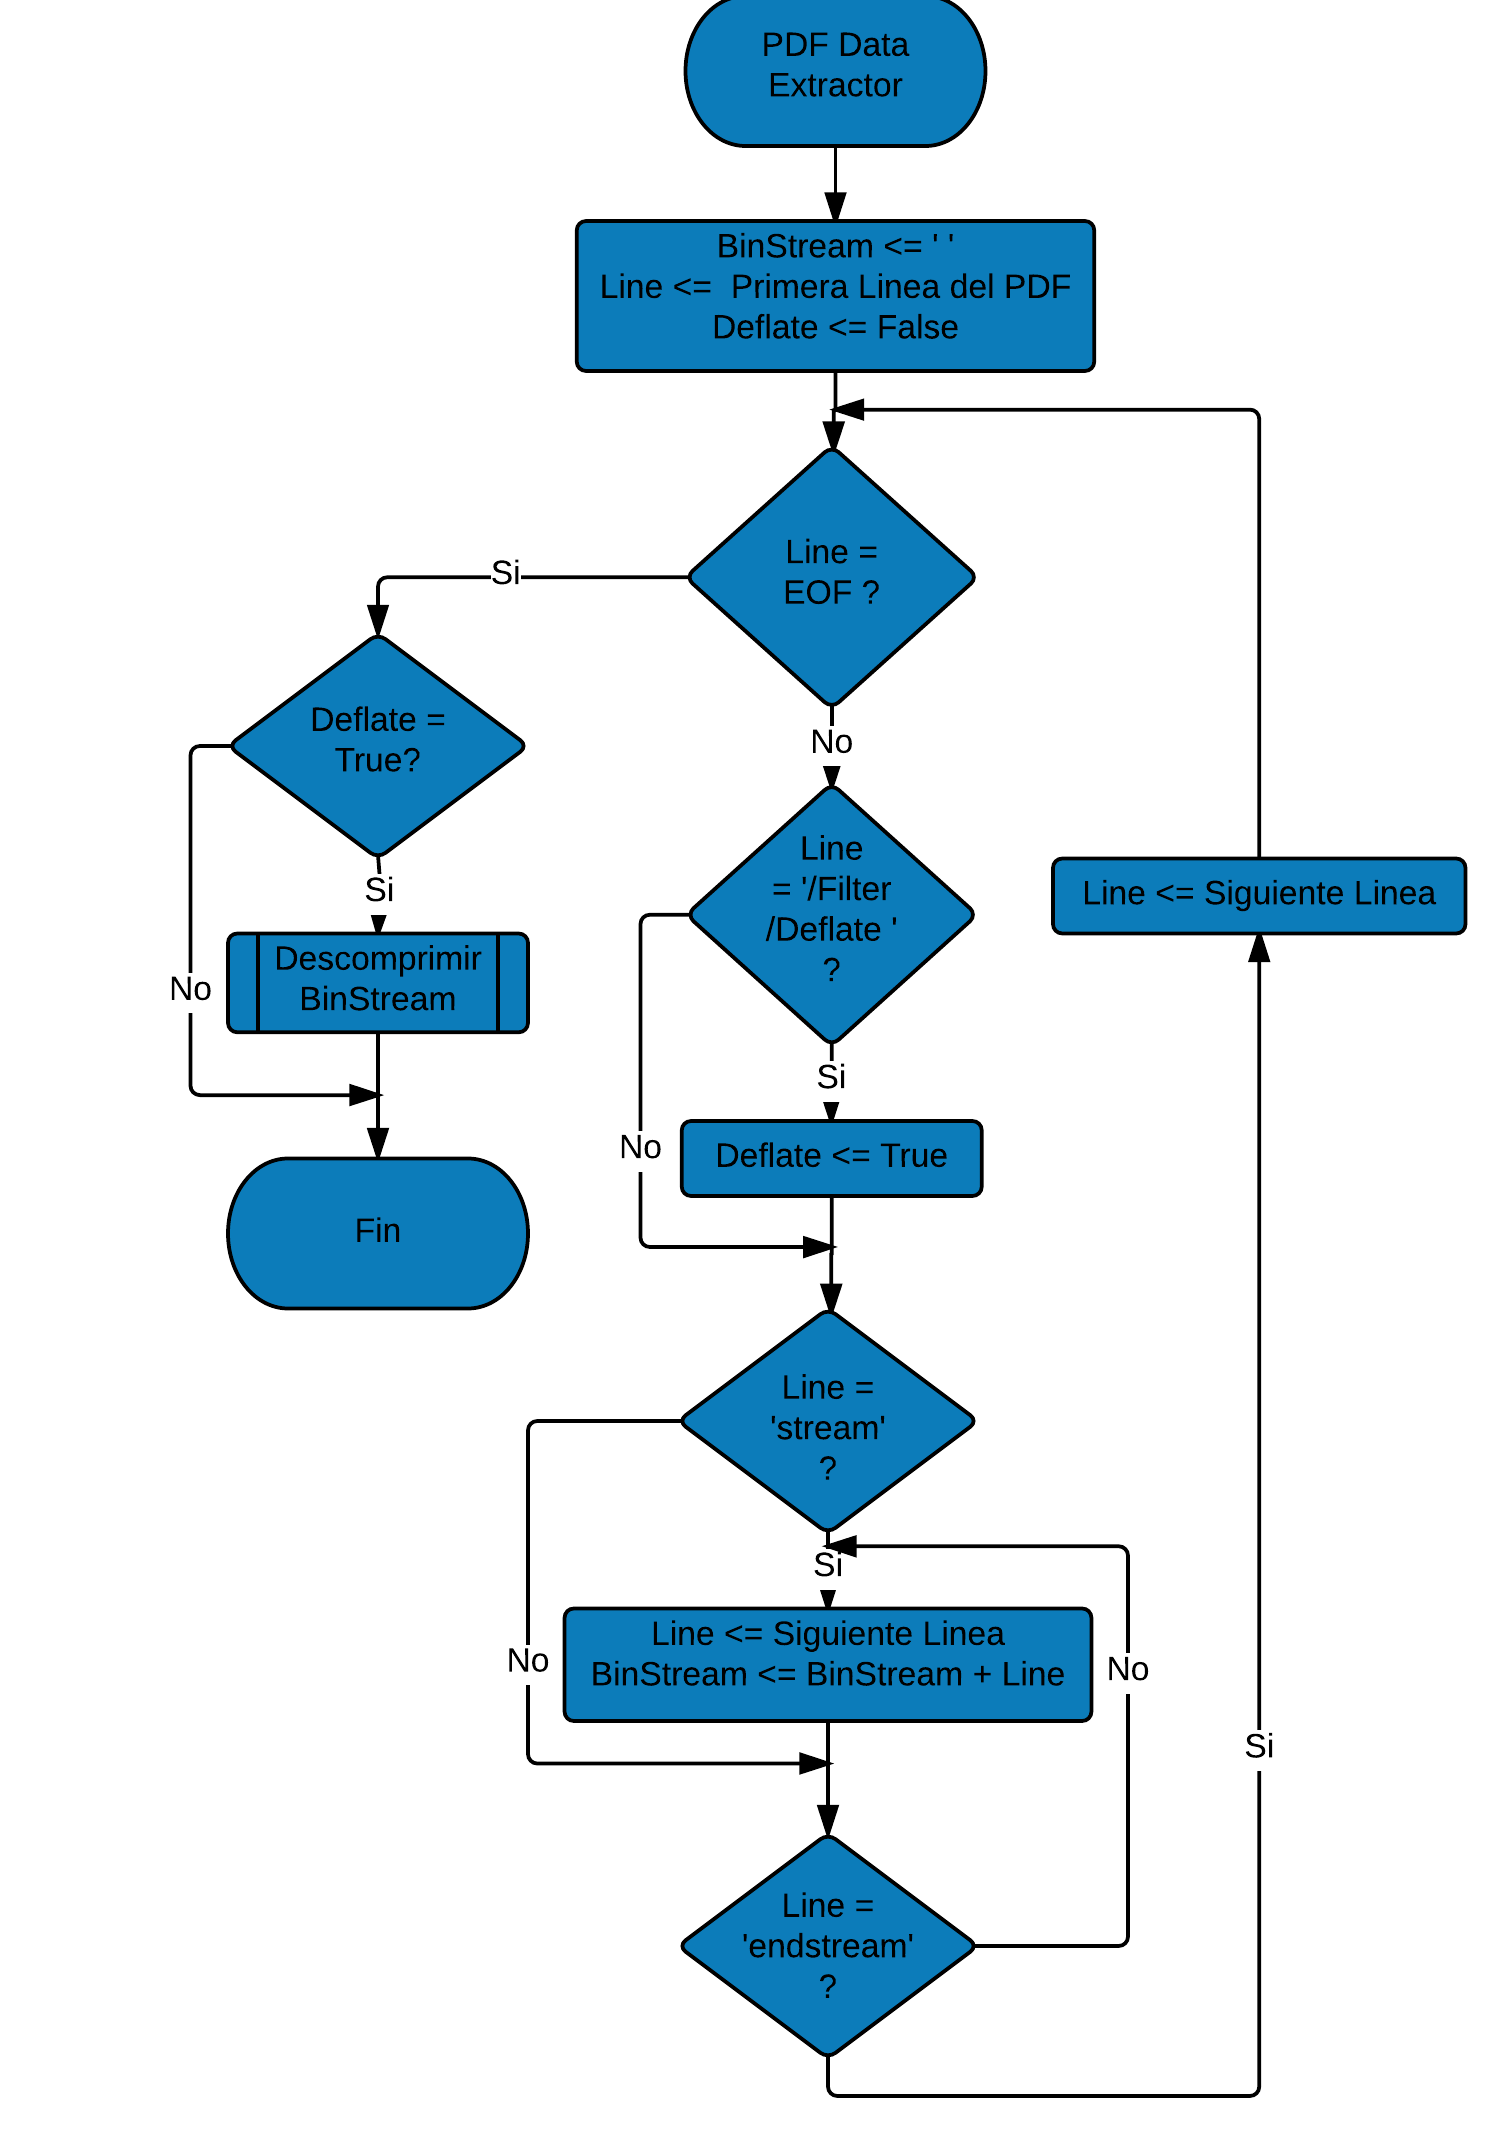
\includegraphics[width=0.7\linewidth]{./Figuras/PDF_Data_Extractor}
        \caption{Programa Extractor de Datos del PDF} 
        \label{Extractor}
\end{figure}

Para implementar el programa se decidi� crear una clase llamada PdfDataExtractor, la clase cuenta con dos miembros FilePath y BinStream.

\begin{minipage}{\linewidth}    
        \begin{lstlisting}[language=Python, caption=Programa Extractor de Datos Del PDF] 
        class PdfDataExtractor(object):
    def __init__(self, file_path):
        self.FilePath = file_path
        self.BinStream = ''     
    \end{lstlisting}
\end{minipage}

FilePath es una variable de tipo string que guarda la localizaci�n del archivo PDF y BinStream es una variable que guarda el script PS extra�do como un string de caracteres Ascii.       

La clase cuenta con ademas con 3 m�todos SetFilePath, GetFilePath y Extract.

El m�todo SetFilePath toma como entrada un string con la localizaci�n de un archivo PDF en el sistema de archivos del sistema operativo y lo guarda como el nuevo valor de FilePath. El m�todo GetFilePath regresa como valor de retorno un string con el valor actual de FilePath y el m�todo Extract implementa el algoritmo principal de la figura \ref{Extractor}. 

A continuaci�n se presenta la implementacion del m�todo Extract.
        \begin{lstlisting}[language=Python, caption=Implementaci�n del Programa Extractor de Datos Del PDF] 
        
    def Extract(self):
        pdfFileObj = open(self.FilePath,'rb')
                
                # This Flag determines if the stream must be decompressed       
        Deflate = False
       
        # Extract the binary stream from the pdf
        for line in pdfFileObj:
            if line == '   /Filter /FlateDecode\n':
                Deflate = True
            if (line == 'stream\n'):
                line = pdfFileObj.next()
                while (line !='endstream\n'):
                    self.BinStream = self.BinStream + line
                    line = pdfFileObj.next()
        pdfFileObj.close()
        # Deflate binary stream if necesary
        if Deflate:
            DeflatedStream = zlib.decompress(self.BinStream)
        else:
            DeflatedStream = self.BinStream
        return DeflatedStream   
        
        
    \end{lstlisting}

\section{Parser de PS a Estructura de Datos Vectoriales}
El siguiente programa auxiliar es el parser de PS, una estructura de datos. Este programa es el encargado de tomar las operaciones contenidas en el script de PS extra�do por el programa extractor de datos y las interpreta de tal forma que sea posible generar los vectores que constituyen el gr�fico vectorial.  
Para generar los vectores, se decidi� utilizar el sistema de programaci�n absoluto ya que este es el  sistema utilizado por las operaciones en PS.

Se tom� como referencia para la creaci�n de los vectores, la esquina superior izquierda del archivo PDF, adem�s se tom� el eje X positivo hacia la derecha del punto cero y el eje Y positivo hacia abajo del punto de referencia.
En la figura \ref{PDF_Parser} se muestra el dise�o del parser, el programa toma como par�metro de entrada el script PS mediante la variable DeflatedStream y retorna como salida todos los vectores que forman el gr�fico.

El programa utiliza dos estructuras de datos internas, la primera se denomin� current\_ path puesto que representa una lista de todos los vectores que forman el gr�fico, la segunda estructura se denomin� VectorCut ya que representa los vectores que ser�n utilizados para realizar el corte con la cortadora l�ser. 
 
Adicionalmente, los comandos PS utilizan una sintaxis postfix por lo que se decidi� utilizar una arquitectura de pila, para ello se utiliz� una pila denominada operands\_ stack.
Finalmente, para la creaci�n de los vectores se utilizaran dos variables extras: Starting Position que representa el punto inicial del path y CurrentPosition que representa el punto final del path.  

El parser toma cada elemento guardado en la variable DeflatedStream, si el elemento es un operando, este es empujado hacia la pila, si el elemento es un operador el parser llama a la subrutina adecuada.

A cada operador PS se le asign� una subrutina particular, cada subrutina define la creaci�n de uno o m�s vectores, al final de cada subrutina, el programa agrega los vectores a Current\_ Path.

\begin{figure}[!htb]
        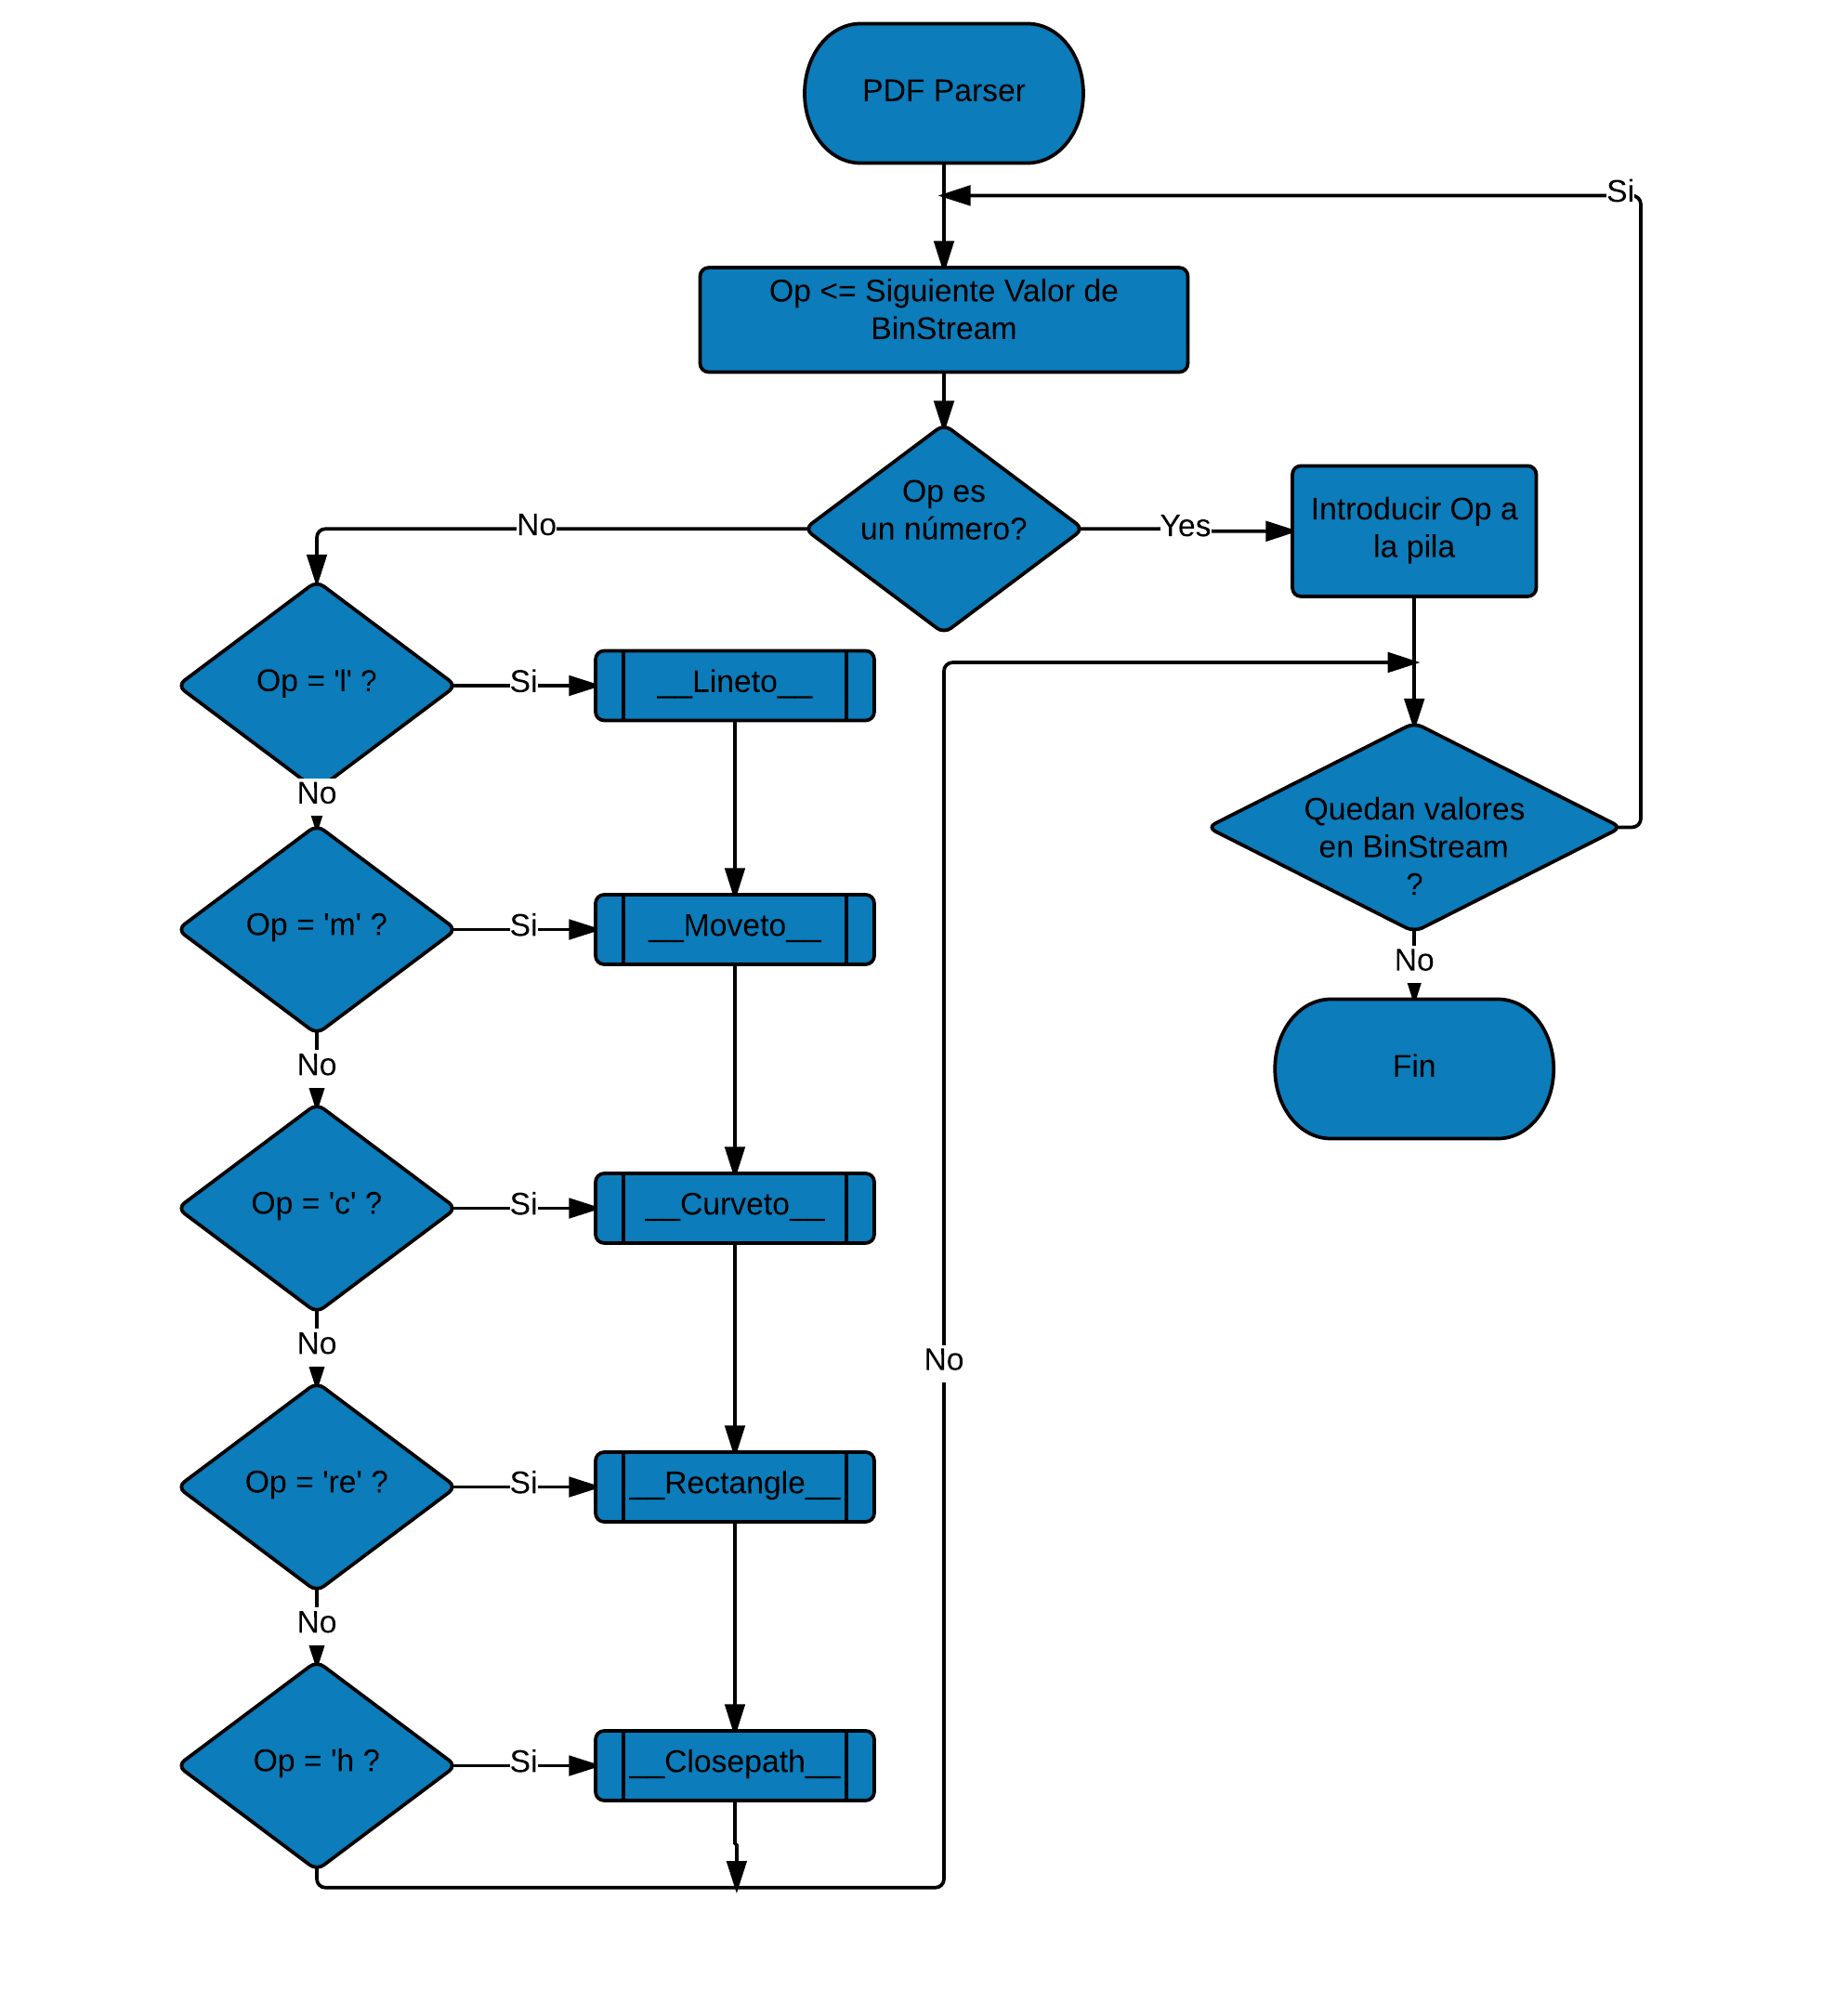
\includegraphics[width=0.9\linewidth]{./Figuras/PDF_Parser}
        \caption{Parser de PDF a Estructura de Datos Vectoriales} 
        \label{PDF_Parser}
\end{figure}

\subsection{Clase VectorCut}
Para la implementaci�n del parser se crearon varias clases, la primera clase llamada VectorCut, es la estructura de datos principal del parser.

Esta clase posee 5 miembros: StartingPoint, EndingPoint, LaserPower, DeltaX y DeltaY.
        
\begin{minipage}{\linewidth}    
        \begin{lstlisting}[language=Python, caption=Clase VectorCut] 
class VectorCut(object):
    # Constructor
    def __init__(self, start=[0.0, 0.0], end=[0.0, 0.0], power=0.0):
        self._StartingPoint_ = start
        self._EndingPoint_ = end
        self._LaserPower_ = power
        self._DeltaX_ = abs((self.__EndingPoint__[0] - self.__StartingPoint__[0]))
        self._DeltaY_ = abs((self.__EndingPoint__[1] - self.__StartingPoint__[1]))
    \end{lstlisting}
\end{minipage}

StartingPoint y EndingPoint representan el punto de inicial y el punto final del vector respectivamente, ambas variables son del tipo lista, el primer elemento de la lista representa la posici�n en la coordenada X del punto, mientras que el segundo elemento representa la posici�n Y del punto. La variable LaserPower representa el porcentaje de potencia que ser� utilizado para realizar el corte, finalmente las variables DeltaX y DeltaY representan la distancia de separaci�n entre los puntos inicial y final, DeltaX en el eje X y DeltaY en el eje Y.  
  
Adicionalmente, la clase incluye un m�todo llamado scale que permite a la clase escalar el vector. El m�todo recibe como entrada un n�mero en punto flotante y multiplica cada elemento de las listas EndingPoint y StartingPoint por este n�mero.  

\begin{minipage}{\linewidth}    
        \begin{lstlisting}[language=Python, caption=Clase VectorCut] 
    def ScaleVector(self, Scale=1.0):
        self.__StartingPoint__[0] *= Scale
        self.__StartingPoint__[1] *= Scale
        self.__EndingPoint__[0] *= Scale
        self.__EndingPoint__[1] *= Scale
    \end{lstlisting}
\end{minipage}

\subsection{Clase CutterPath}
La siguiente clase se llama CutterPath, esta clase representa el path formado por los vectores de corte, a continuaci�n se muestra el c�digo implementado.   

\begin{minipage}{\linewidth}    
        \begin{lstlisting}[language=Python, caption=Clase CutterPath] 
class CutterPath(object):
    def __init__(self):
        self.__Queue__ = deque([])
    \end{lstlisting}
\end{minipage}

Se eligi� una cola como la estructura de datos utilizada, ya que se requiere que los cortes se realicen en el orden dictado por el archivo PDF. Para implementar esta funcionalidad se utiliz� el contenedor de python deque. La clase cuenta con 3 m�todos: el m�todo add a�ade un vector al final de la lista, el m�todo pop elimina el primer elemento de la lista y lo regresa como valor de retorno y finalmente el m�todo len regresa un n�mero entero que representa cuantos vectores forman el camino. 

\begin{minipage}{\linewidth}    
        \begin{lstlisting}[language=Python, caption=M�todos de CutterPath] 
    # Length of the path, how many vectors form the path
    def __len__(self):
        return len(self.__Queue__)
    # Add a vector to the path
    def add(self, Vector):
        self.__Queue__.append(Vector)
    # Remove a Vector from the path
    def pop(self):
        return self.__Queue__.popleft()
    \end{lstlisting}
\end{minipage}
  
  
\subsection{Clase PostScriptInterpreter}
Finalmente se cre� una clase llamada PostScriptInterpreter, esta clase implementa el algoritmo de la figura \ref{PDF_Parser}, la clase cuenta con 5 miembros: OperandsStack, CurrentPosition, StartingPosition, CurrentPath y Power.
  
\begin{minipage}{\linewidth}    
        \begin{lstlisting}[language=Python, caption=Clase PostScriptInterpreter.] 
def __init__(self, power=0.0):
        self.OperandsStack = []
        self.CurrentPosition  = [0.0, 0.0]
        self.StartingPosition = [0.0, 0.0]
        self.__CurrentPath__ = CutterPath()
        self.__Power__ = power
    \end{lstlisting}
\end{minipage}

Operands\_ stack es una instancia del objeto lista de python, para utilizarla con la funcionalidad de pila se emplearon los m�todos append que agrega un elemento al final de la lista y pop que retorna el �ltimo elemento de la lista. StartingPosition y CurrentPosition siguen la nomenclatura utilizada hasta este momento para definir puntos, se utiliz� una lista con 2 elementos. En los archivos PDF el path siempre comienza por el punto de origen, por lo que las variables StartingPosition y CurrentPosition tomar�n el valor inicial de [0.0, 0.0].
es la pila que fue utilizada para guardar los operandos, CurrentPosition es una lista que contiene la posici�n final del �ltimo vector creado por el programa, StartingPosition guarda la posici�n inicial del primer vector que forma el path, CurrentPath es una instancia de la clase CutterPath, est� es la encargada de de guardar los vectores que forman el path que va a ser cortado y finalmente la variable Power representa el porcentaje de potencia que va a ser utilizado en el corte. 

La clase cuenta con un m�todo llamado IsFloat que se encarga revisar si el elemento obtenido de DeflatedStream es o no un n�mero.  

\begin{minipage}{\linewidth}    
        \begin{lstlisting}[language=Python, caption=M�todo IsFloat.] 
    def __IsFloat__(self, value):
        try:
            float(value)
            return True
        except:
            return False
    \end{lstlisting}
\end{minipage}

El m�todo principal de la clase PostScriptInterpreter se llama Operate, este m�todo es el encargado de llamar a las subrutinas que generan los vectores de corte dependiendo del operador recibido.   
        \begin{lstlisting}[language=Python, caption=M�todo principal de la clase PostScriptInterpreter: Operate.] 
    def Operate(self, Op):
        if self.__isfloat__(Op):
            self.OperandsStack.append(Op)
        else:
            # Create a Square
            if Op == 're':
                self.__Square__()
            # Moveto
            elif Op == 'm':
                self.__Moveto__()
            # Lineto
            elif Op == 'l':
                self.__Lineto__()
            # Curveto
            elif Op == 'c':
                self.__Curveto__()
            # Close Current Path
            elif Op == 'h':
                self.__ClosePath__()
            else:
                print 'Do nothing'
    \end{lstlisting}

Se dise�� una subrutina para cada operador PS que afecta el path, a continuaci�n se discutir�n a fondo cada una de estas subrutinas.

La primera subrutina se llama Lineto y es la encargada de interpretar el operador del mismo nombre, la subrutina saca los dos primeros operandos del Stack y forma un punto con ellos, luego crea un VectorCut que utiliza la posici�n actual como punto inicial, el punto generado como punto final adem�s y utiliza el valor de la variable Power para definir el valor de la potencia del corte.  

\begin{minipage}{\linewidth}    
        \begin{lstlisting}[language=Python, caption=M�todo Lineto] 
def __Lineto__(self):
        YMovement= float(self.OperandsStack.pop())
        XMovement= float(self.OperandsStack.pop())
        self.CurrentPath.append(VectorCut(self.CurrentPosition, [XMovement, YMovement], self.__Power__))
        self.CurrentPosition = [XMovement, YMovement]
    \end{lstlisting}
\end{minipage}

La siguiente subrutina se llama Moveto, esta subrutina saca los dos primeros operandos del Stack y forma un punto con ellos, luego crea un VectorCut que utiliza la posici�n actual como punto inicial, el punto generado como punto final  y utiliza una potencia de corte igual a cero.  

\begin{minipage}{\linewidth}    
        \begin{lstlisting}[language=Python, caption=M�todo Moveto] 
    def __Moveto__(self):
        YMovement= float(self.OperandsStack.pop())
        XMovement= float(self.OperandsStack.pop())
        self.CurrentPath.append(VectorCut(self.StartingPosition, [XMovement, YMovement], 0.0))
        self.CurrentPosition = [XMovement, YMovement]
        self.StartingPosition = [XMovement, YMovement]
    \end{lstlisting}
\end{minipage}

La siguiente subrutina se llama ClosePath, esta subrutina se encarga de cerrar el path actual creando un VectorCut iniciando en CurrentPosition y terminando en StartingPosition.   

\begin{minipage}{\linewidth}    
        \begin{lstlisting}[language=Python, caption=M�todo ClosePath.] 
    def __ClosePath__(self):
        self.CurrentPath.append(VectorCut(self.CurrentPosition, self.StartingPosition, self.__power__))
        self.CurrentPosition = self.StartingPosition
        \end{lstlisting}
\end{minipage}

La subrutina Square toma los par�metros, height, width, X, y Y de la pila y crea 4 puntos que representa las 4 esquinas del rect�ngulo:

\begin{enumerate}
        \item La esquina inferior izquierda [X,Y]
        \item La esquina inferior derecha   [(X + width), Y]
        \item La esquina superior derecha   [(X + width), (Y + height)]
        \item La esquina superior izquierda [X , (Y + height)]
\end{enumerate} 

Luego crea cinco vectores, el primero un vector de movimiento que va desde el CurrentPoint hasta el punto 1 y cuatro vectores que pasan por cada una de las cuatro esquinas del rect�ngulo en el orden establecido arriba, finalizando de nuevo en el punto 1. 

\begin{minipage}{\linewidth}    
        \begin{lstlisting}[language=Python, caption=M�todo Square.] 
        def __Square__(self):
        square_height = float(self.OperandsStack.pop())
        square_width  = float(self.OperandsStack.pop())
        square_Y0     = float(self.OperandsStack.pop())
        square_X0     = float(self.OperandsStack.pop())
        Point1 = [square_X0, square_Y0]
        Point2 = [square_X0+square_width, square_Y0]
        Point3 = [square_X0+square_width, square_Y0+square_height]
        Point4 = [square_X0, square_Y0+square_height]
        self.CurrentPath.append(VectorCut(self.CurrentPosition, Point1))
        self.CurrentPath.append(VectorCut(Point1, Point2, self.__power__))
        self.CurrentPath.append(VectorCut(Point2, Point3, self.__power__))
        self.CurrentPath.append(VectorCut(Point3, Point4, self.__power__))
        self.CurrentPath.append(VectorCut(Point4, Point1, self.__power__))
        self.CurrentPosition = Point1
        \end{lstlisting}
\end{minipage}

La �ltima subrutina es la subrutina Curveto, este m�todo toma de la pila los cuatro puntos de control necesarios para generar la curva c�bica de B�zier y utiliza las formulas \ref{Eq:Bezier1} y \ref{Eq:Bezier2} para producir una curva con cien puntos.

La subrutina aplica un algoritmo de interpolaci�n lineal para unir los puntos generados con las ecuaciones de B�zier con l�neas rectas.

El algoritmo funciona uniendo dos puntos consecutivos de la curva mediante un VectorCut.
A continuaci�n se muestra la implementaci�n de esta subrutina:

\begin{minipage}{\linewidth}    
        \begin{lstlisting}[language=Python, caption=M�todo Square.] 
        def __Curveto__(self):
        # Starting Point
        Y0= self.CurrentPosition[1]
        X0= self.CurrentPosition[0]
        # Ending Point
        Y3= float(self.OperandsStack.pop())
        X3= float(self.OperandsStack.pop())
        # Bezier Control Points
        Y2= float(self.OperandsStack.pop())
        X2= float(self.OperandsStack.pop())
        Y1= float(self.OperandsStack.pop())
        X1= float(self.OperandsStack.pop())
        # Setup the parametrization
        number_of_points = 100
        t = scipy.linspace(0, 1, number_of_points)
        # Use the Bezier formula
        Bx = (1-t)**3*X0 + 3*(1-t)**2*t*X1 + 3*(1-t)*t**2*X2 + t**3*X3
        By = (1-t)**3*Y0 + 3*(1-t)**2*t*Y1 + 3*(1-t)*t**2*Y2 + t**3*Y3
        bpc = 0  # Bezier Point Counter
                #Bezier Vector Generator
        for point in t:
            xpos = Bx[bpc]
            ypos = By[bpc]
            CurrentPos = [xpos, ypos]
            tempVector = VectorCut(self.CurrentPosition, CurrentPos, self.__power__)
            self.CurrentPath.append(VectorCut(self.CurrentPosition, CurrentPos, self.__power__))
            self.CurrentPosition = CurrentPos
            bpc += 1
        self.CurrentPosition = [X3, Y3]
        \end{lstlisting}
\end{minipage}

\section{Generador de Programas CNC}
El siguiente programa desarrollado fue el Generador de Programas CNC, este programa est� encargado de tomar el path generado por el parser de PS a estructura de datos vectoriales y generar el programa CNC que ser� cargado en la cortadora l�ser.

El programa toma como entradas el path mediante la variable Path y el nombre del archivo de salida mediante la variable OutputFile.

En la figura \ref{generador_cnc} se presenta un diagrama de flujo con el dise�o del programa CNC, el programa toma cada Vector contenido en la variable Path y guarda el punto inicial en las variables $Y_0$ y $X_0$ adem�s de guardar el punto final en las variables $Y_f$ y $X_f$. Luego llama a la subrutina XYInterpolation para generar los comandos de corte.

Al finalizar, se crea un archivo con el nombre recibido por medio de la variable OutputFile y en ella se escriben el header y los comandos de corte.   

\begin{figure}[!htb]
        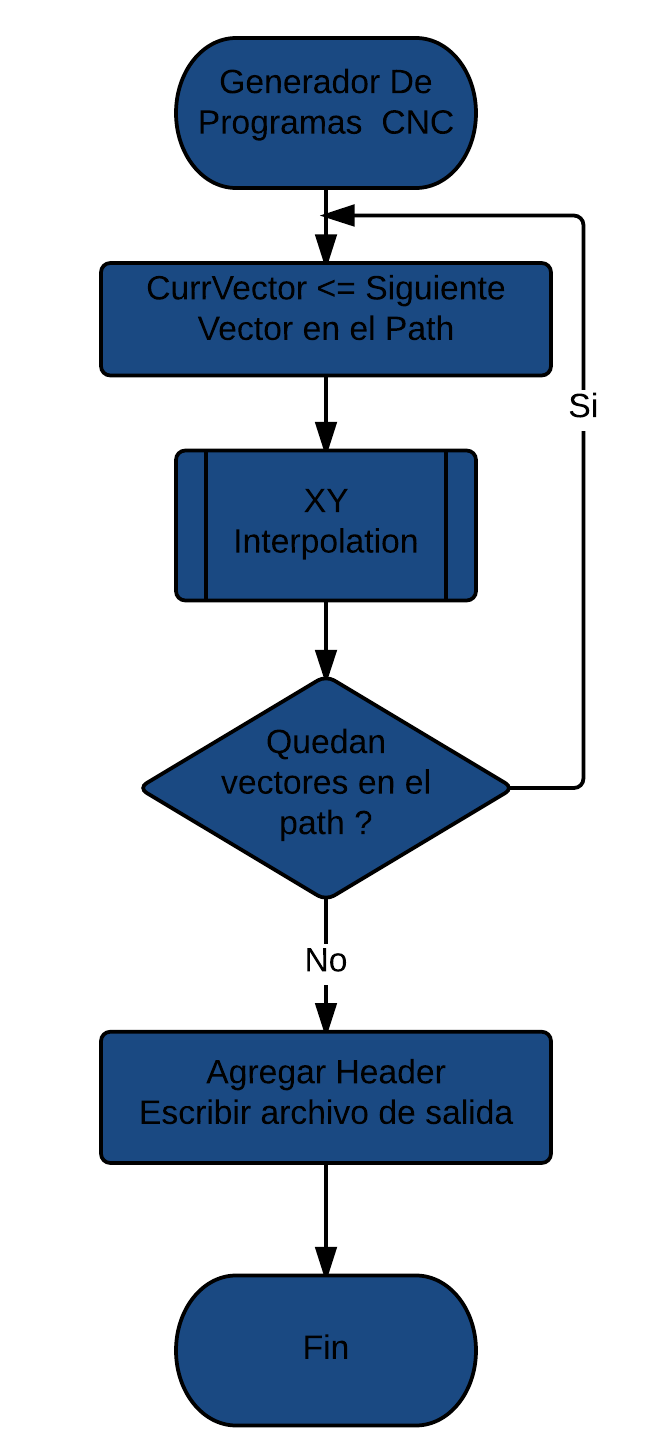
\includegraphics[width=0.3\linewidth]{./Figuras/generador_cnc}
        \caption{Parser de PDF a Estructura de Datos Vectoriales} 
        \label{generador_cnc}
\end{figure}

La figura \ref{XYInterpolation} muestra un diagrama de flujo con el dise�o la subrutina XYInterpolation, 
est� subrutina hace uso del  algoritmo de interpolaci�n lineal descrito en \cite{RoboticsAge}. 

\begin{figure}[!htb]
        \includegraphics[width=0.5\linewidth]{./Figuras/Interpolation}
        \caption{Algoritmo de Interpolaci�n Lineal XY.} 
        \label{XYInterpolation}
\end{figure}

El algoritmo se puede resumir en los siguientes pasos los siguientes pasos:

\begin{enumerate}
        \item El primer paso es definir los puntos de programaci�n inicial y el final.
        \item Se calcula la direcci�n del eje X con la ecuaci�n \ref{Eq:Delta X}. 
        \item Se calcula la direcci�n del eje Y con la ecuaci�n \ref{Eq:Delta Y}.
        \item Si Dx es positivo el byte de signo para los movimientos en el eje X es 0x00 de caso contrario es 0x01. 
        \item Si Dy es positivo el byte de signo para los movimientos en el eje Y es 0x00 de caso contrario es 0x02. 
        \item Se utiliza la ecuaci�n \ref{Eq:FXY} para calcular el valor de la variable FXY. 
        \item Si el valor de FXY es negativo, se agrega un step en el eje Y. Y se agrega el valor de $|DX|$ a FXY.  
        \item Si el valor de FXY es positivo, se agrega un step en el eje X. Y se agrega el valor de $|DY|$ a FXY.  
        \item Este proceso se repite hasta que cabezal de la cortadora alcance la posici�n $[X_f,Y_f]$.
\end{enumerate}

A continuaci�n se presentan las ecuaciones utilizadas por el algoritmo.

\begin{equation}
        \label{Eq:Delta X}      
        Dx = X_f - X_0
\end{equation}

\begin{equation}
        \label{Eq:Delta Y}      
        Dy = Y_f - Y_0
\end{equation}

\begin{equation}
        \label{Eq:FXY}  
        FXY = |Dx| - |Dy|
\end{equation}

\subsubsection{Clase CncGenerator} 
Para implementar el programa generador de archivos CNC se crearon 2 clases, la primera clase se denomin� 
CncGenerator, esta clase cuenta con 2 miembros: Path y OutputFile.
Path es una variable que guarda el Path creado por el programa Parser mientras que OutputFile guarda un string con el nombre que se le desee dar al programa CNC generado.

\begin{minipage}{\linewidth}    
        \begin{lstlisting}[language=Python, caption=Clase CncGenerator.] 
class CncGenerator(object):
        def __init__(self, path, output_file, speed):
        self._Path_ = path
        self._OutputFile_ = output_file
        \end{lstlisting}
\end{minipage}

El m�todo principal de esta clase se llama Execute, el cual es el encargado de implementar el algoritmo de la figura \ref{generador_cnc}. Se utiliza la librer�a copy para generar una copia de los vectores que son extra�dos de la variable path llamada CurrVector, debido a que python utiliza las variables por referencia. 

Adicionalmente se utiliza el m�todo ScaleVector con una escala de 0.0139, esto se debe a que los vectores generados por el programa parser utilizan el pixel como unidad de mediada y los gr�ficos cuentan con una resoluci�n de 72 pixeles por pulgada (PPI) \citep{adobe2005pdf}. Mientras que la cortadora l�ser necesita de 1000 steps para realizar un corte de una pulgada. \citep{Alex}
    
\begin{minipage}{\linewidth}    
        \begin{lstlisting}[language=Python, caption=M�todo Execute.] 
def Execute(self):
        for Vector in range(len(self._Path_)):
                        # Make A Copy Of the Vector to be Executed
            CurrVector = copy.deepcopy(self._Path_.pop())
            
                        # Convert it from PPI to inches.             
            CurrVector.ScaleVector(1.0/72.0)
            
            # make the cut commands             
            cut = CommandsGenerator(CurrVector)
            commands = cut._XYInterpolation_() 
                        
                        print('Vector number {} executed').format(Vector + 1)
     
                # makes and stores the fullpacket in job using the libjob library
        laser_bin = lj.jobPacket(commands)
        laser_bin.makePacket()
        job = laser_bin.getBin()
        # the job is written to a file
        with open(self._OutputFile_, 'a') as bin:
            bin.write(job)
        bin.close()
            
        \end{lstlisting}
\end{minipage}

\subsubsection{Clase CommandsGenerator}
La clase CommandsGenerator implementa el algoritmo de la figura \ref{XYInterpolation}, cuenta con dos miembros Vector y commands. 

Vector es una variable para guardar el vector recibido y commands es una variable tipo string  hexadecimal que guarda los comandos los comandos generados. 

\begin{minipage}{\linewidth}    
        \begin{lstlisting}[language=Python, caption=Clase CommandsGenerator.] 
class CommandsGenerator(object):
    def _ init_ (self, VectorCut):
        self.CurrentVector = VectorCut
        self.commands = ''
        \end{lstlisting}
\end{minipage}

La clase cuenta con 3 m�todos, get\_ power, cut\_ command y XYInterpolation.  
El primer m�todo llamado get\_ power utiliza la ecuaci�n \ref{Eq:Power} para calcular el valor del byte de potencia de cada comando de corte.

\begin{minipage}{\linewidth}    
        \begin{lstlisting}[language=Python, caption= M�todo getpower.] 
    def _ get_ power_ (self):
        PD = self.CurrentVector.GetLaserPower()
        P=int(PD*(255.0/100.0))
        return chr(P)
        \end{lstlisting}
\end{minipage}

El segundo m�todo se llama cut\_ command y es el encargado de formar el comando de corte utilizando las variables Sign, StpX, StpY y la salida del m�todo get\_ power. 

\begin{minipage}{\linewidth}    
        \begin{lstlisting}[language=Python, caption= M�todo cutcommand.] 
    def _ cut_command_(self, Sign, Stp_X, Stp_Y):
        self.commands += '{}{}{}{}'.format(Sign, Stp_ X, Stp_Y, self._ get_ power_())
        \end{lstlisting}
\end{minipage}

Finalmente el m�todo XYInterpolation implementa la subrutina del mismo nombre, el m�todo utiliza la funci�n de python chr para convertir n�meros enteros en strings hexadecimales para formar los comandos del programa CNC.   

\begin{minipage}{\linewidth}    
        \begin{lstlisting}[language=Python, caption= Configuraci�n de las variables utilizadas por el m�todo XYInterpolation.]  
    def _XYInterpolation_(self):
        # current position is set to the starting position
        X0 = self.Current_Vector.Get_Start()[0]
        Y0 = self.Current_Vector.Get_Start()[1]
        Xf = self.Current_Vector.Get_End()[0]
        Yf = self.Current_Vector.Get_End()[1]
        # current position is set to the starting position
        X = X0
        Y = Y0
        # X Axis direction, if the value of DX is positive, the laser move to
        # the rigth if the value is negative the laser move to the left.
        DX = Xf - X0
        SignX = chr(0)
        SignY = chr(0)
        if DX >= 0:
            StepX = 1
            SignX = chr(1)
        else:
            StepX = -1
        # Y Axis direction, if the value of DY is positive, the laser move down
        # if the value is negative the laser up.
        DY = Yf - Y0
        if DY >= 0:
            StepY = 1
        else:
            StepY = -1
            SignY = chr(2)
        # Current function symbol, if FXY is greater than or equal to zero, the
        # laser must move in the X axis, else the laser move in the Y axis
        FXY = math.fabs(DX) - math.fabs(DY)
        \end{lstlisting}
\end{minipage}

\begin{minipage}{\linewidth}    
        \begin{lstlisting}[language=Python, caption= Lazo principal del m�todo XYInterpolation.] 
        # Main loop:
        while not ((X == Xf) and (Y == Yf)):
            if FXY >= 0:
                X += StepX
                FXY -= math.fabs(DY)
                self._cut_command_(SignX, '\x01', '\x00')
            else:
                Y += StepY
                FXY += math.fabs(DX)
                self._cut_command_(SignY, '\x00', '\x01')
        \end{lstlisting}
\end{minipage}

\section{Software de Cortado}
El �ltimo programa desarrollado consiste en el software de cortado, este programa hace uso de los programas anteriores para producir el corte a partir del gr�fico vectorial guardado en el archivo PDF.

El programa toma cuatro par�metros por parte del usuario: La direcci�n del archivo PDF del que se desea extraer el gr�fico vectorial, la direcci�n IP de la cortadora l�ser, el porcentaje de la potencia m�xima que se desea utilizar para realizar el corte y el nombre del archivo de salida.
En la figura \ref{Programa_Corte} se muestra un diagrama de flujo con el dise�o del algoritmo del software de cortado.

\begin{figure}[!htb]
        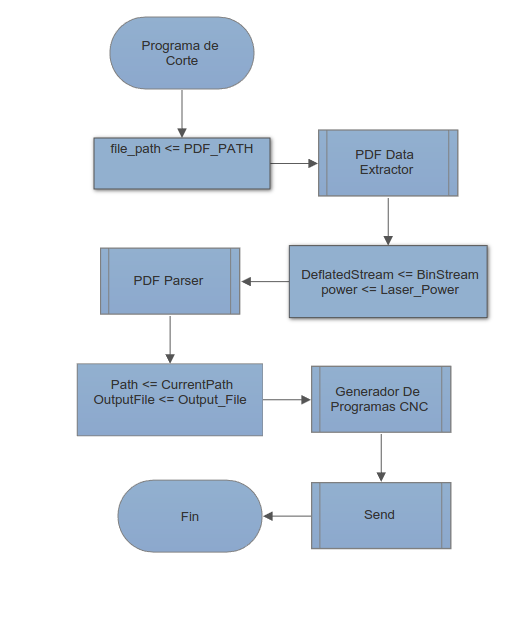
\includegraphics[width=0.5\linewidth]{./Figuras/Programa_Corte}
        \caption{Software de Cortado} 
        \label{Programa_Corte}
\end{figure}


El programa le env�a la direcci�n del archivo pdf al extractor de datos mediante la variable file\_ Path, y recibe la salida de este por medio de una variable llamada DeflatedStream. 
Luego le envi� al programa PDF parser la potencia del l�ser mediante la variable power, el script PS extraido mediante la variable DeflatedStream y recibe la salida de este mediante la variable Path.

A continuaci�n el programa de corte le env�a al programa generador de CNC, las variables Path y OutputFile para producir el programa CNC.

Finalmente el programa llama a una subrutina llamada Send que es la encargada de enviar el programa CNC a la 
cortadora l�ser por medio del protocolo de comunicaci�n descrito en la secci�n \ref{sec:L2.3.4}.  
Para este programa se cre� una GUI, el dise�o se aprecia en la figura. En el ap�ndice \ref{apex1} se discute a profundidad el uso de la interfaz gr�fica.  

\begin{figure}[!htb]
        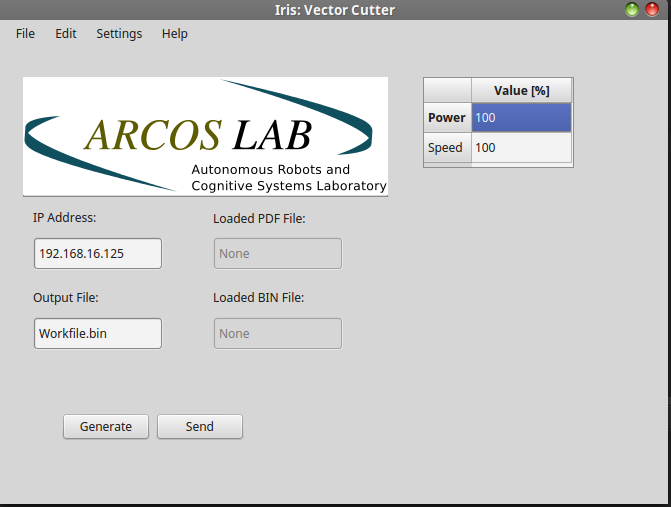
\includegraphics[width=0.5\linewidth]{./Figuras/GUI}
        \caption{GUI del software de cortado.} 
        \label{GUI}
\end{figure}

\chapter{Resultados} \label{sec:L04}
Para probar el funcionamiento de los programas desarrollados se realizaron varios escenarios de prueba.

El primer escenario fue la realizaci�n de diversos cortes en l�nea recta, el prop�sito de esta prueba fue comprobar el funcionamiento del algoritmo de interpolaci�n lineal y del m�todo lineto.

En la figura \ref{Test5} se observan los distintos cortes realizados por la cortadora l�ser.

\begin{figure}[!htb]
        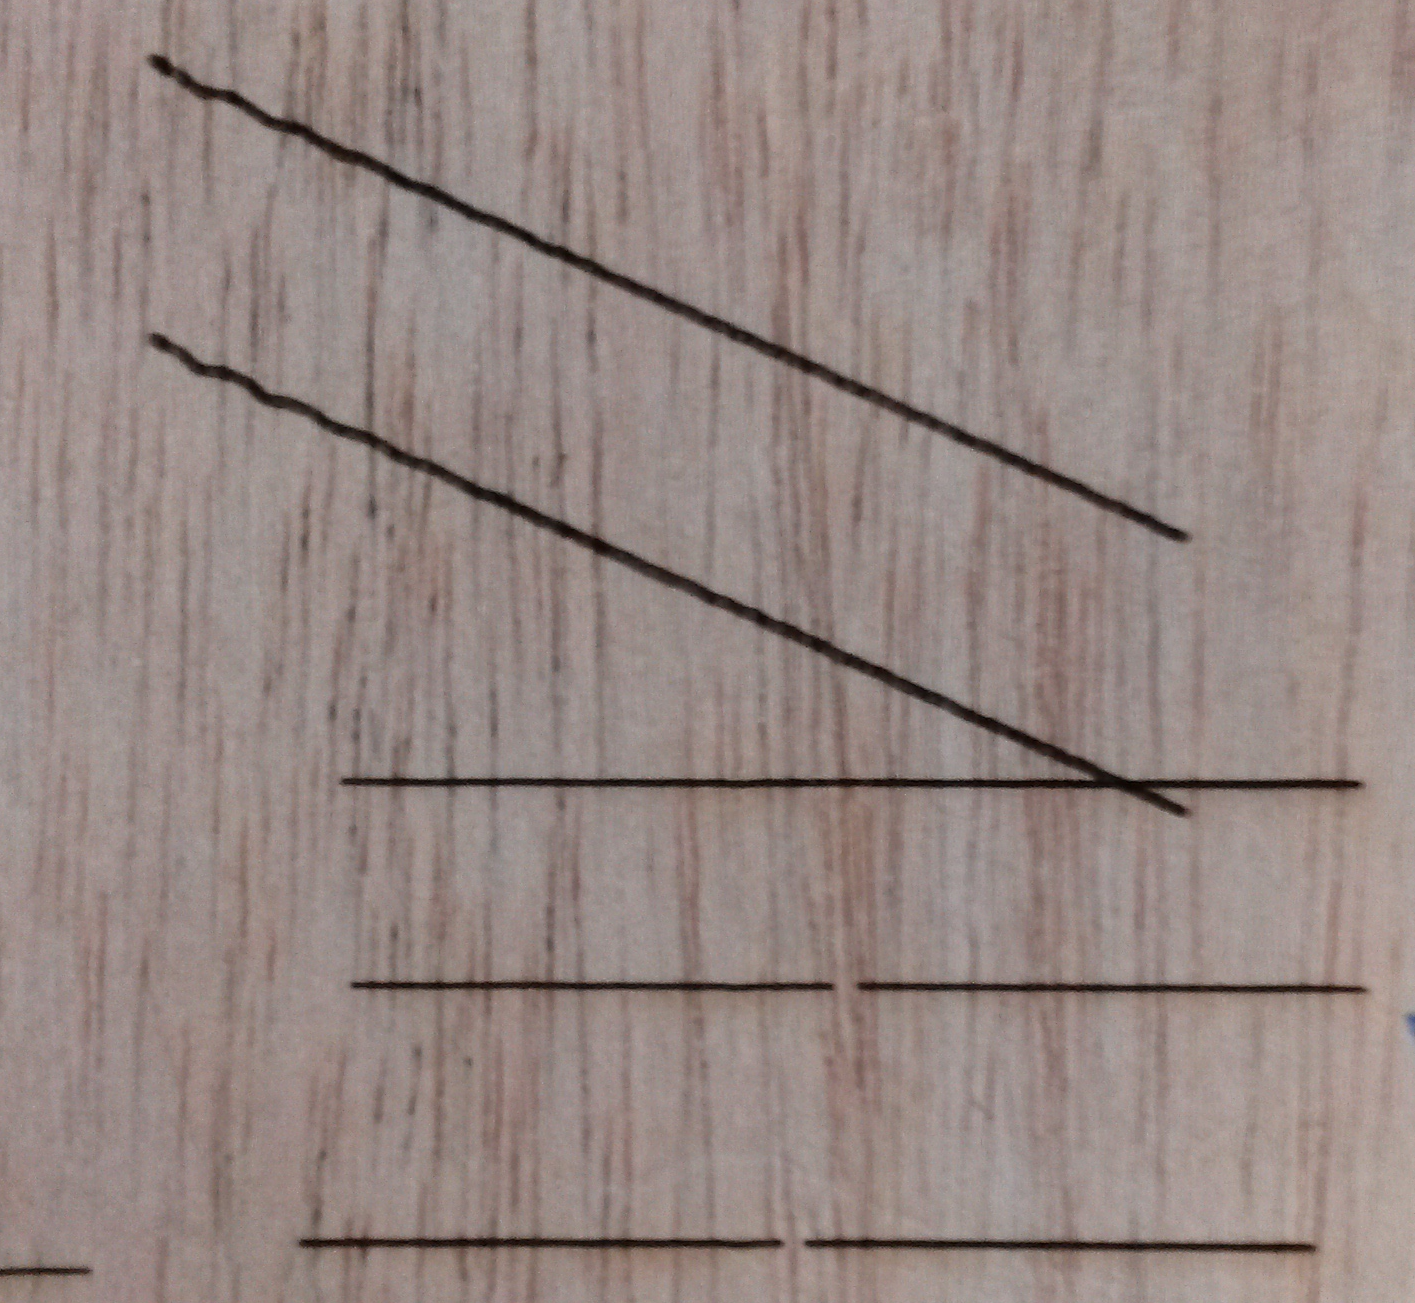
\includegraphics[width=0.3\linewidth]{./Figuras/Test5}
        \caption{Cortes realizados para la prueba 1.} 
        \label{Test5}
\end{figure}

El segundo escenario de prueba fue la realizaci�n de un corte en curva, el prop�sito de esta prueba fue comprobar el funcionamiento del m�todo Curveto. 

En la figura \ref{Test_pdf_4} se tiene la imagen PDF generada para realizar la prueba, en la figura \ref{Test_figure_4} se muestra una representaci�n gr�fica de los vectores generados y en la figura \ref{Test4} se observa el corte realizado por la cortadora l�ser.

\begin{figure}[!htb]
        
\includegraphics[width=0.3\linewidth]{./Figuras/Test_pdf_4}
        \caption{Imagen PDF utilizada para la prueba 2.} 
        \label{Test_pdf_4}
\end{figure}

\begin{figure}[!htb]
        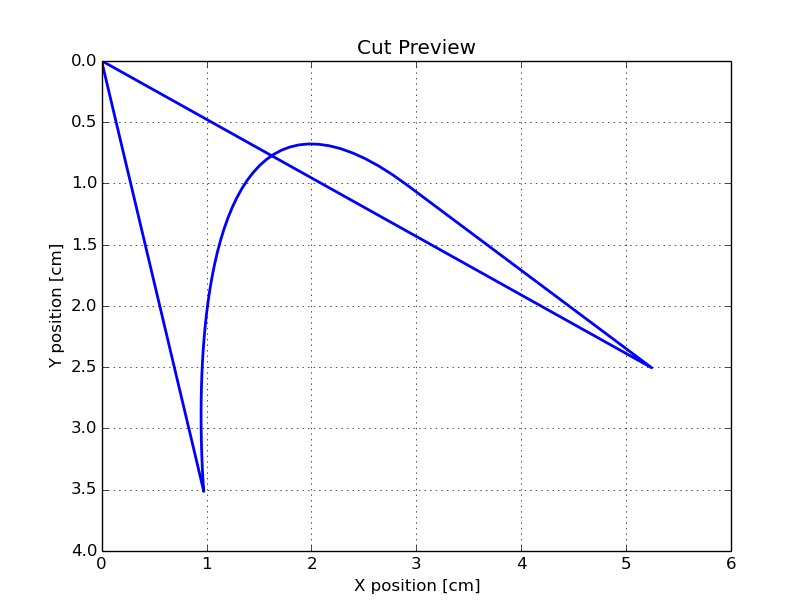
\includegraphics[width=0.5\linewidth]{./Figuras/Test_figure_4}
        \caption{Vectores Generados para la prueba 2} 
        \label{Test_figure_4}
\end{figure}

\begin{figure}[!htb]
        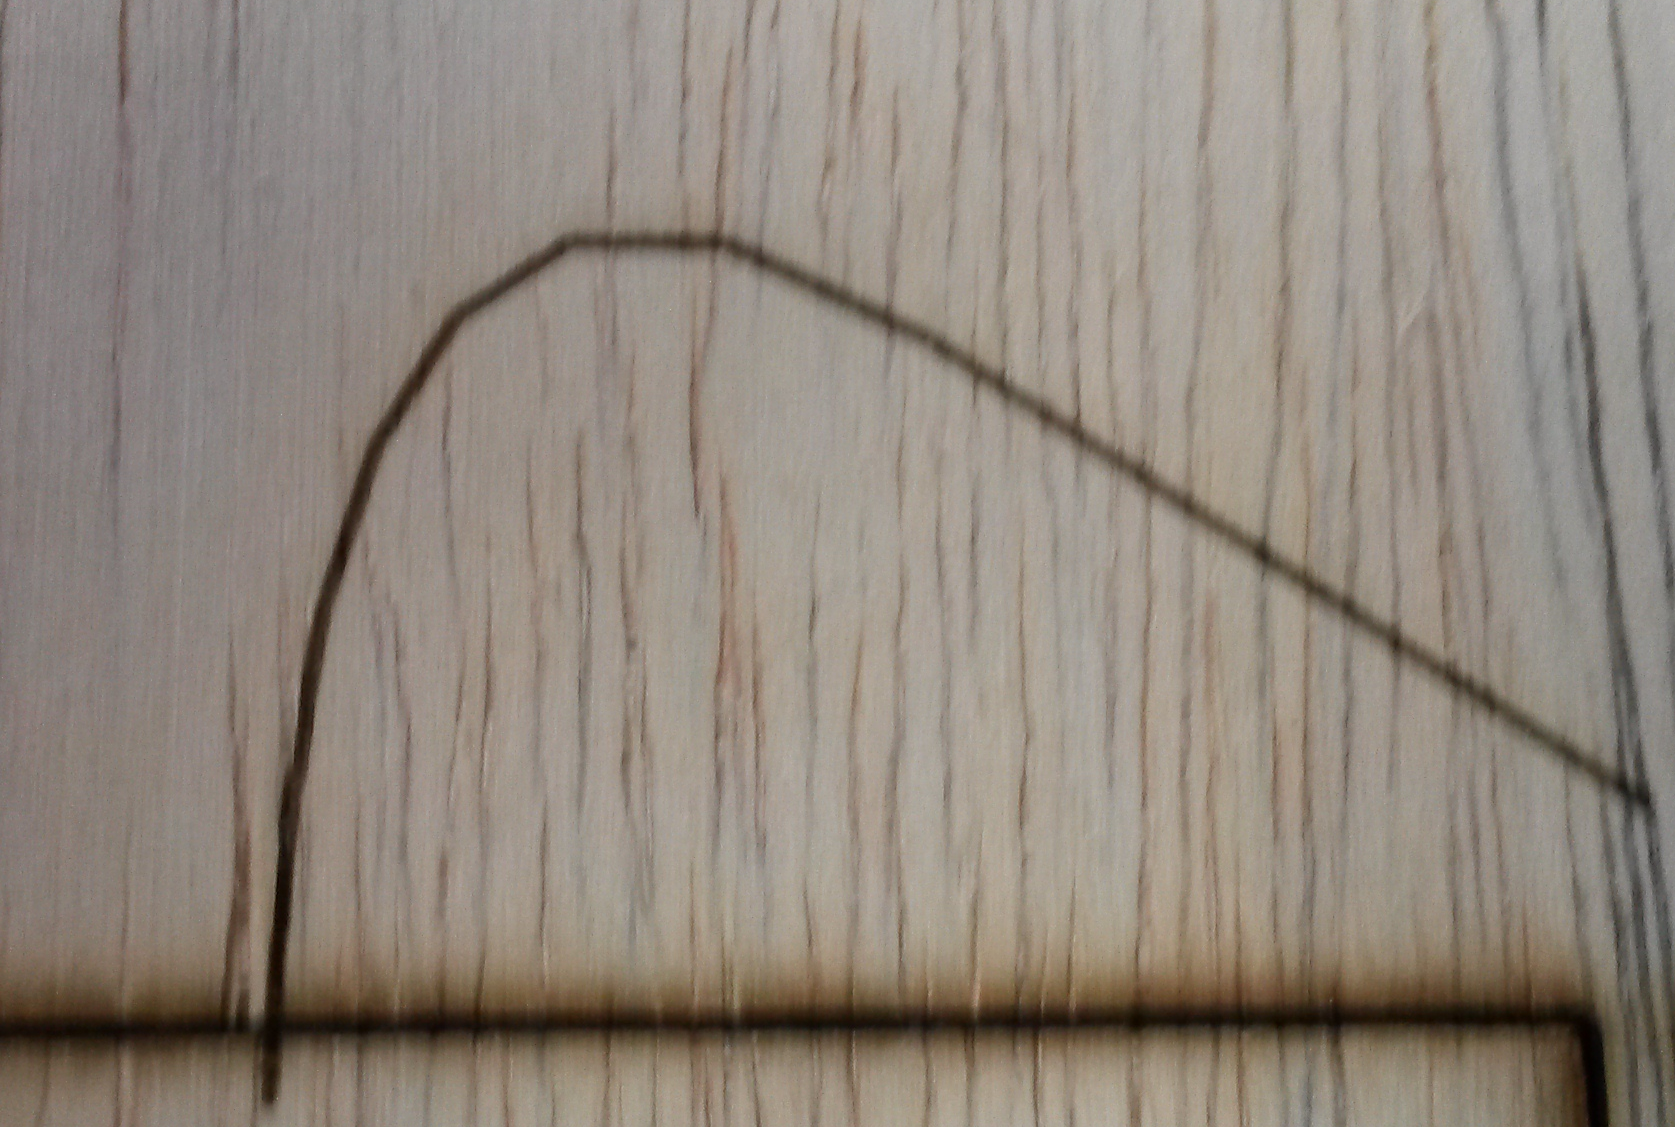
\includegraphics[width=0.3\linewidth]{./Figuras/Test4}
        \caption{Corte Realizado en la prueba 2} 
        \label{Test4}
\end{figure}

El tercer escenario de prueba fue la realizaci�n de un corte rectangular, en este caso la intenci�n fue la de comprobar el funcionamiento del m�todo Rectangule.    

En la figura \ref{Test_pdf_3} se tiene la imagen PDF generada para realizar la prueba, en la figura \ref{Test_figure_3} se muestra una representaci�n gr�fica de los vectores generados y en la figura \ref{Test3} se observa el corte realizado por la cortador� l�ser.

\begin{figure}[!htb]
        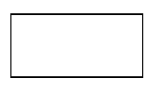
\includegraphics[width=0.3\linewidth]{./Figuras/Test_PDF_3}
        \caption{Imagen PDF utilizada para la prueba 3.} 
        \label{Test_pdf_3}
\end{figure}

\begin{figure}[!htb]
        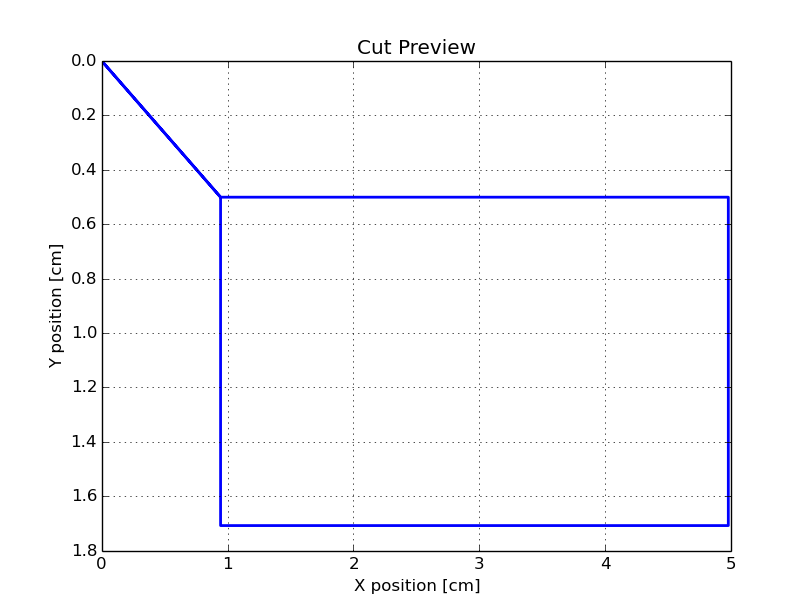
\includegraphics[width=0.5\linewidth]{./Figuras/Test_figure_3}
        \caption{Vectores Generados para la prueba 3} 
        \label{Test_figure_3}
\end{figure}

\begin{figure}[!htb]
        
\includegraphics[width=0.3\linewidth]{./Figuras/Test3}
        \caption{Corte Realizado en la prueba 3} 
        \label{Test3}
\end{figure}

El cuarto escenario de prueba fue la realizaci�n de un corte que consiste en una espiral y un pent�gono, el prop�sito de esta prueba fue comprobar el comportamiento de la cortadora al realizar varios curvetos de forma consecutiva.  

En la figura \ref{Test_pdf} se tiene la imagen PDF generada para realizar la prueba, en la figura \ref{Test_figure_1} se muestra una representaci�n gr�fica de los vectores generados y en la figura \ref{Test} se observa el corte realizado por la cortadora l�ser.

\begin{figure}[!htb]
        
\includegraphics[width=0.3\linewidth]{./Figuras/Test_pdf}
        \caption{Imagen PDF utilizada para la prueba 4.} 
        \label{Test_pdf}
\end{figure}

\begin{figure}[!htb]
        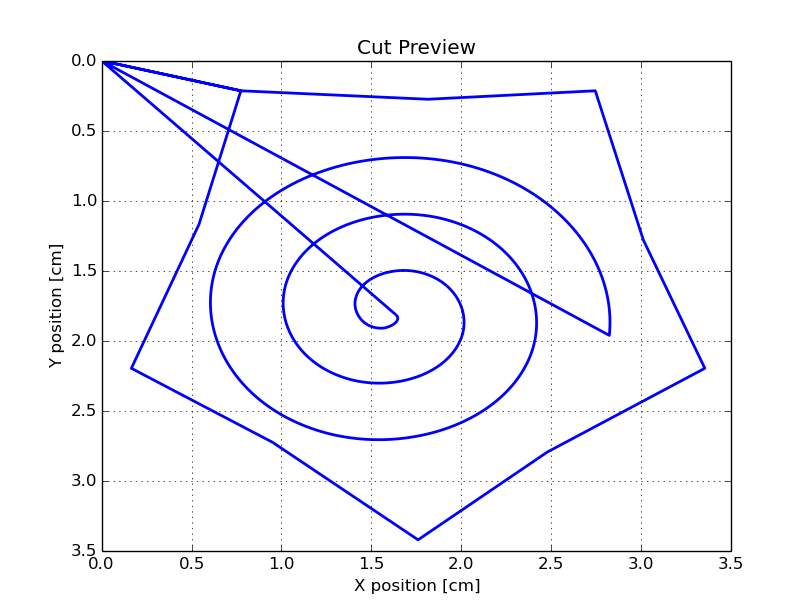
\includegraphics[width=0.5\linewidth]{./Figuras/Test_figure_1}
        \caption{Vectores Generados para la prueba 4.} 
        \label{Test_figure_1}
\end{figure}

\begin{figure}[!htb]
        
\includegraphics[width=0.3\linewidth]{./Figuras/Test}
        \caption{Corte Realizado en la prueba 4.} 
        \label{Test}
\end{figure}

El �ltimo escenario de prueba consisti� en realizar el corte de un archivo layout, el prop�sito de esta prueba fue comprobar el comportamiento de la cortadora con archivo de complejidad real.

En la figura \ref{Test_pdf_6} se tiene la imagen PDF generada para realizar la prueba, en la figura \ref{Test_figure_6} se muestra una representaci�n gr�fica de los vectores generados y en la figura \ref{Test6} se observa el corte realizado por la cortadora l�ser.

\begin{figure}[!htb]
        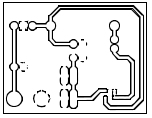
\includegraphics[width=0.3\linewidth]{./Figuras/Test_PDF_6}
        \caption{Imagen PDF utilizada para la prueba 5.} 
        \label{Test_pdf_6}
\end{figure}

\begin{figure}[!htb]
        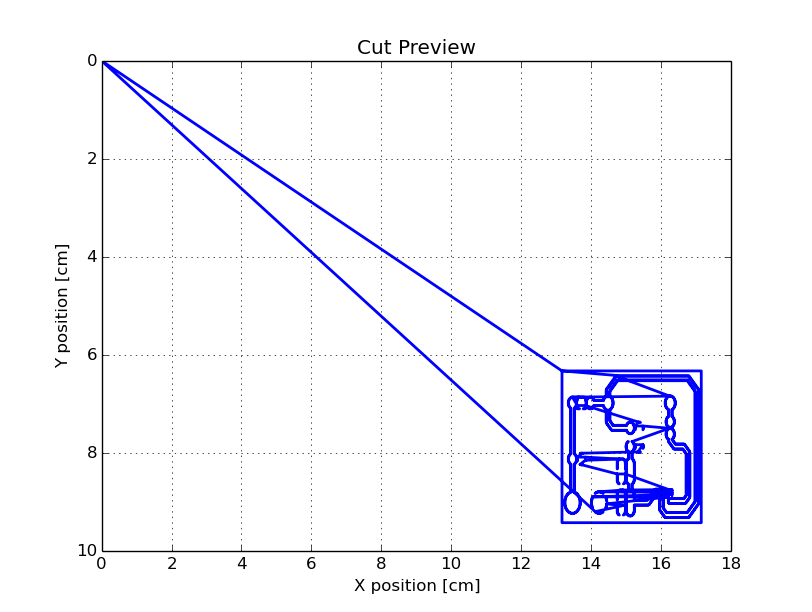
\includegraphics[width=0.5\linewidth]{./Figuras/Test_figure_6}
        \caption{Vectores Generados para la prueba 5.} 
        \label{Test_figure_6}
\end{figure}

\begin{figure}[!htb]
        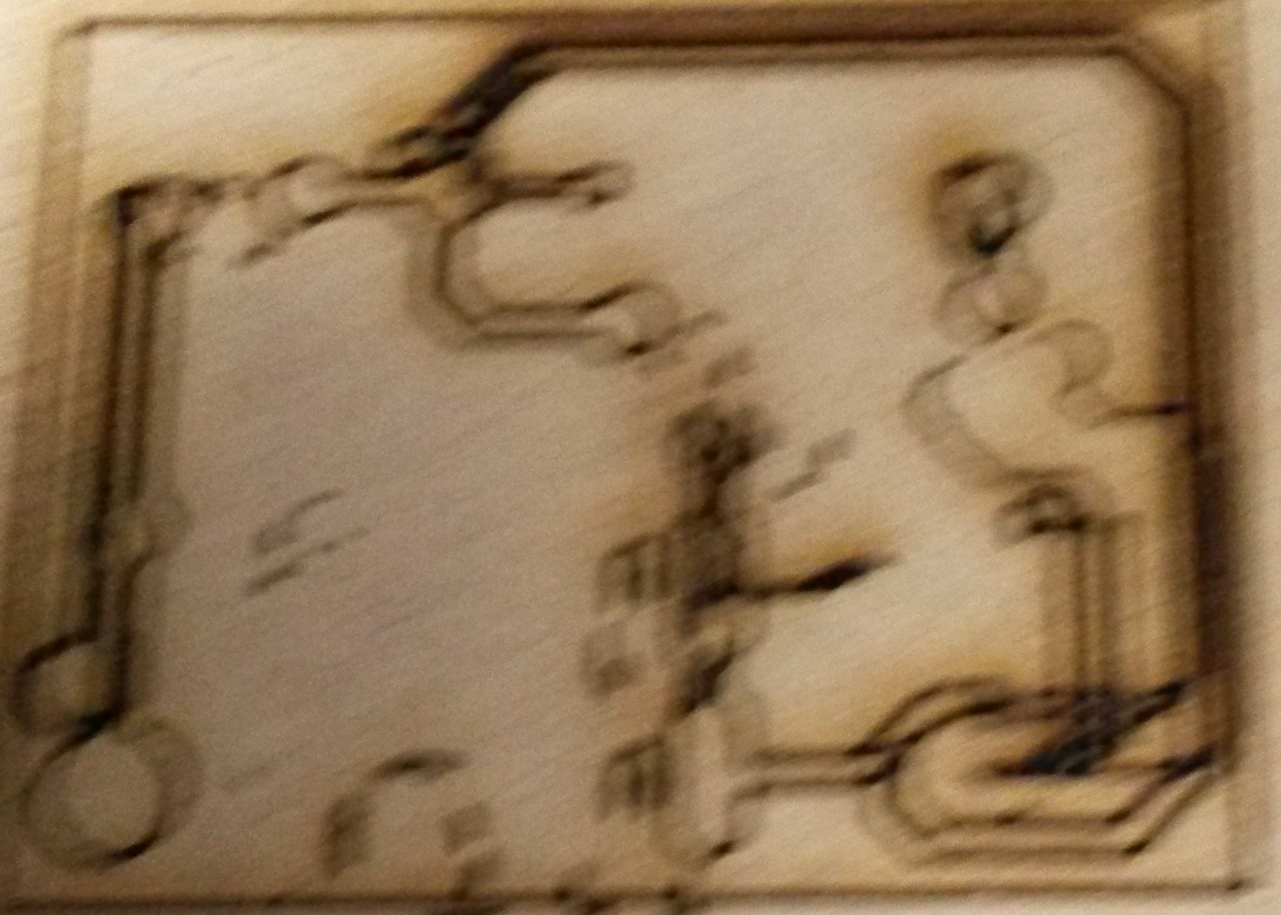
\includegraphics[width=0.3\linewidth]{./Figuras/Test6}
        \caption{Corte Realizado en la prueba 5} 
        \label{Test6}
\end{figure}
 
%-----------------------------
\chapter{Conclusiones y recomendaciones} \label{sec:L05}
\subsection{Conclusiones}

\begin{enumerate}
        \item Se logr� documentar el protocolo de comunicaci�n de la cortadora l�ser "Laser Spectrum H-Series 20x12 5th Gen " y se consigui� realizar una conexi�n entre la cortadora l�ser y una computadora con el sistema operativo GNU/Linux.
        \item Se dise�� un software de cortado que permite tomar un archivo PDF y transformarlo en comandos de corte para la cortadora "Laser Spectrum H-Series 20x12 5th Gen ".
        \item Se realiz� implementaci�n del software de cortado en el lenguaje de programaci�n Python, adem�s de realizar la implementaci�n de todos los programas auxiliares necesarios para el funcionamiento del software dise�ado.
        \item El dise�o propuesto consiste en diversos m�dulos independientes entre s� lo que permite que el cada m�dulo sea modificado por separado lo que facilita que sea modificado en el futuro.
        \item Se realizaron diversas pruebas de funcionamiento lo que permiti� comprobar el desempe�o de los distintos algoritmos implementados.     
\end{enumerate}

\subsection{Recomendaciones }
\begin{enumerate}
        \item En la �ltima prueba realizada, en la figura \ref{Test6} se observan algunos bugs al realizar el corte del archivo layout, el archivo layout fue producido utilizando un gr�fico rasterizado que fue convertido a un gr�fico vectorial por medio de la herramienta Inkscape. El an�lisis preliminar del script extra�do con el programa PDF Extract sugiere que la cortadora pierde la referencia luego de realizar un comando h. Por lo que se recomienda ampliar la implementaci�n de la subrutina closepath.     
        \item Se realiz� una cobertura funcional de los programas realizados, por lo que se recomienda desarrollar una metodolog�a para realizar un an�lisis cuantitativo de los resultados obtenidos. Por ejemplo implementar un simulador de la cortadora l�ser para comparar la salida del simulador con los vectores producidos por el programa Parser y as� calcular alguno de los �ndices de error.  

\end{enumerate}

%\subsection{Trabajo Futuro}
%\begin{enumerate}
%       \item 
%       \item
%       \item
%\end{enumerate}

%\subsection{Trabajo Futuro}

%== POR USUARIO (BIBLIOGRAF�A) --------------------------------------
%estilo de la bibliograf�a (formato APA modificado para espa�ol)
%nombre del archivo con la bibliograf�a (.bib)
\bibliography{eieclases_ref}
\cleardoublepage

%== POR USUARIO (AP�NDICES) -----------------------------------------
%ap�ndices, si es que los hay
% si no hay, comentar la siguiente l�nea con % para que no aparezcan
%\appendix

%archivo de ap�ndice si fuera necesario
%archivo del Ap�ndice

\chapter{Ap�ndices} \label{apex}

\section{Ap�ndice A: Tutorial Uso Del Programa De Corte} \label{apex1}

En este ap�ndice se describe el uso del programa de cortado desarrollado.

En la figura \ref{GUI1} se muestra la interfaz gr�fica.

\begin{figure}[!htb]
        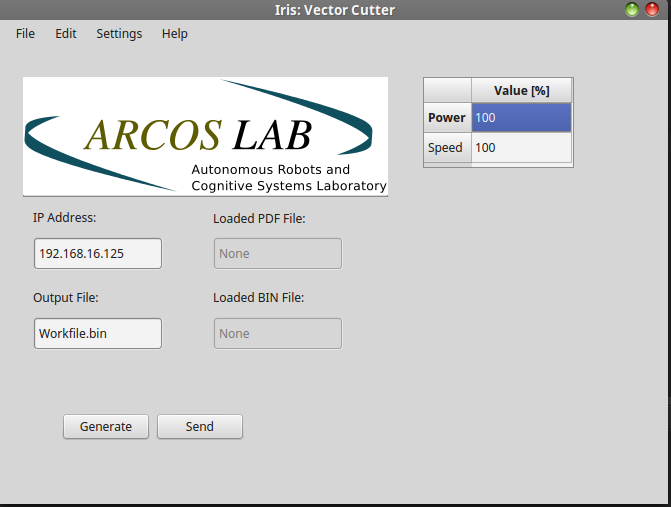
\includegraphics[width=0.5\linewidth]{./Figuras/GUI}
        \caption{GUI del software de cortado.} 
        \label{GUI1}
\end{figure}

El primer paso para realizar el corte es cargar el archivo PDF, para ello se selecciona la opci�n Load PDF en el menu FILE. Esto nos muestra una ventana de dialogo donde podemos seleccionar el archivo PDF deseado como se observa en la figura \ref{GUI2}.

\begin{figure}[!htb]
        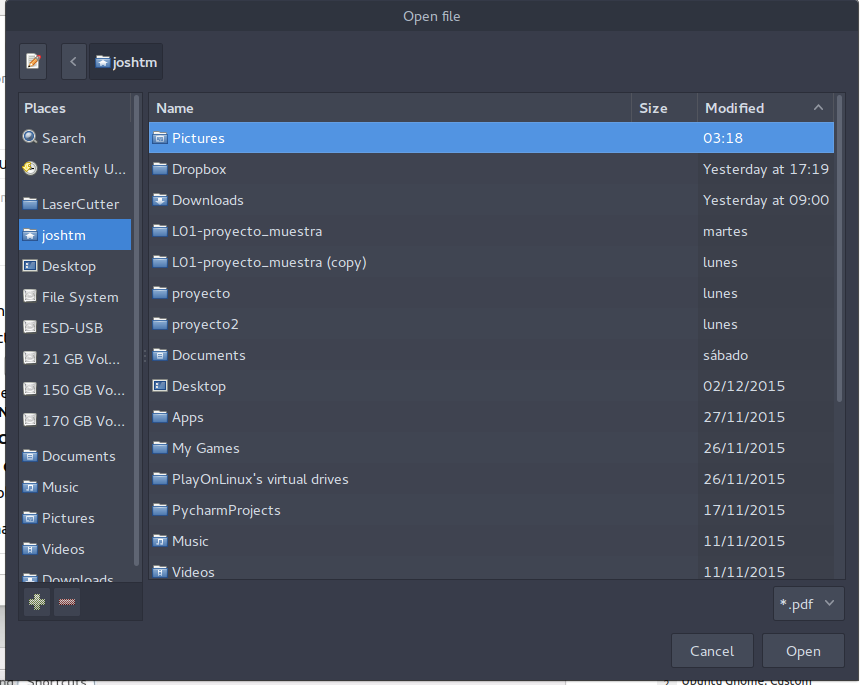
\includegraphics[width=0.5\linewidth]{./Figuras/GUI2}
        \caption{Dialogo de selecci�n de archivo.} 
        \label{GUI2}
\end{figure}

Una vez seleccionado el archivo PDF, su nombre aparece bajo el cuadro Loaded PDF lo cual nos asegura que el archivo fue cargado con �xito.

El siguiente paso es seleccionar un nombre para el archivo de salida, para ello se escribe el nombre deseado y su extensi�n en el cuadro Output File como se observa en la figura \ref{GUI3}. Por default el nombre del archivo es Workfile.bin.

\begin{figure}[!htb]
        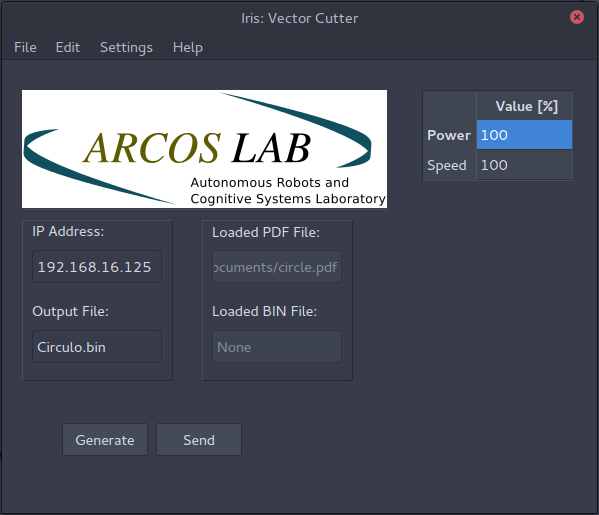
\includegraphics[width=0.5\linewidth]{./Figuras/GUI3}
        \caption{Selecci�n del archivo de salida.} 
        \label{GUI3}
\end{figure}


El siguiente paso es seleccionar una potencia de salida, para ello se cambia el valor de Power en el cuadro localizado en la esquina superior derecha. Una vez hecho esto, se procede a darle click en el bot�n Generate. Al final la creaci�n del archivo de corte aparecer� una ventana con un preview del corte a realizar como se muestra en la figura \ref{GUI4}. 

\begin{figure}[!htb]
        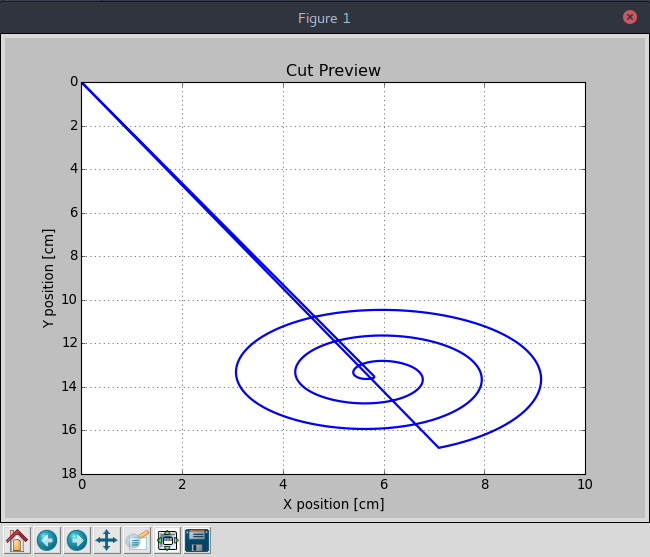
\includegraphics[width=0.5\linewidth]{./Figuras/GUI4}
        \caption{Ventana que contiene un vistazo preliminar del corte.} 
        \label{GUI4}
\end{figure}

Al cerrar esta ventana aparecer� el nombre del archivo de corte cargado en el cuadro Loaded Binary File como se observa en la figura \ref{GUI5}. Si se est� satisfecho con el preview del corte, el siguiente paso es enviarlo a la cortadora l�ser para realizar el corte. 

\begin{figure}[!htb]
        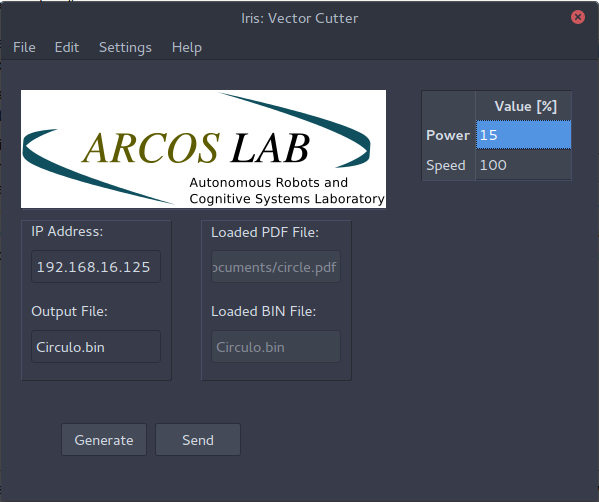
\includegraphics[width=0.5\linewidth]{./Figuras/GUI5}
        \caption{Ventana que contiene un vistazo preliminar del corte.} 
        \label{GUI5}
\end{figure}

Para utilizar la cortadora l�ser es necesario seguir los pasos de seguridad planteados en: \url{https://wiki.arcoslab.eie.ucr.ac.cr/doku.php/internal:cortadora_laser}.

Una vez encendida, la cortadora l�ser indicara su direcci�n IP asignada, este valor deber� ser introducido en el cuadro IP Address. 

El paso final es hacer click en el bot�n Send, si no ocurre ning�n inconveniente, la cortadora comenzar� a realizar el trabajo de corte.  

\clearpage
\newpage

\section{Ap�ndice B: C�digo Completo de la GUI} \label{apex2}

\begin{lstlisting}[language=Python, caption= C�digo Completo de la GUI .]

from PyQt4 import QtCore, QtGui
import os
import VectorCut
import socket

try:
    _fromUtf8 = QtCore.QString.fromUtf8
except AttributeError:
    def _fromUtf8(s):
        return s

try:
    _encoding = QtGui.QApplication.UnicodeUTF8
    def _translate(context, text, disambig):
        return QtGui.QApplication.translate(context, text, disambig, _encoding)
except AttributeError:
    def _translate(context, text, disambig):
        return QtGui.QApplication.translate(context, text, disambig)


class Ui_MainWindow(object):


    def setupUi(self, MainWindow):
        MainWindow.setObjectName(_fromUtf8("MainWindow"))
        MainWindow.resize(661, 480)
        
        self.centralwidget = QtGui.QWidget(MainWindow)
        self.centralwidget.setObjectName(_fromUtf8("centralwidget"))

        # ScrollArea instance
        self.scrollArea = QtGui.QScrollArea(self.centralwidget)

        # ScrollArea image
        self.Output_label = QtGui.QLabel(self.scrollArea)
        self.Output_label.setObjectName(_fromUtf8("Output_label"))
        self.image = QtGui.QPixmap("arcoslabrev3a.png")

        # ScrollArea properties
        self.scrollArea.setGeometry(QtCore.QRect(20, 30, 365, 120))
        self.scrollArea.setWidgetResizable(True)
        self.scrollArea.setObjectName(_fromUtf8("scrollArea"))
        self.scrollAreaWidgetContents = QtGui.QWidget(self.Output_label)
        self.scrollAreaWidgetContents.setGeometry(QtCore.QRect(0, 0, 259, 269))
        self.scrollAreaWidgetContents.setObjectName(_fromUtf8("scrollAreaWidgetContents"))
        self.scrollArea.setWidget(self.scrollAreaWidgetContents)
        # self.scrollArea.setHorizontalScrollBarPolicy(QtCore.Qt.ScrollBarAlwaysOn)
        # self.scrollArea.setVerticalScrollBarPolicy(QtCore.Qt.ScrollBarAlwaysOn)

        # table, takes the config option from the user
        self.tableWidget = QtGui.QTableWidget(self.centralwidget)
        self.tableWidget.setGeometry(QtCore.QRect(420, 30, 151, 91))
        self.tableWidget.setObjectName(_fromUtf8("tableWidget"))
        self.tableWidget.setColumnCount(1)
        self.tableWidget.setRowCount(2)
        item = QtGui.QTableWidgetItem()
        self.tableWidget.setVerticalHeaderItem(0, item)
        item = QtGui.QTableWidgetItem()
        self.tableWidget.setVerticalHeaderItem(1, item)
        item = QtGui.QTableWidgetItem()
        self.tableWidget.setHorizontalHeaderItem(0, item)
        item = QtGui.QTableWidgetItem()
        self.tableWidget.setItem(0, 0, item)
        item = QtGui.QTableWidgetItem()
        self.tableWidget.setItem(1, 0, item)

        # Central frame
        self.frame = QtGui.QFrame(self.centralwidget)
        self.frame.setGeometry(QtCore.QRect(20, 160, 151, 161))
        self.frame.setFrameShape(QtGui.QFrame.StyledPanel)
        self.frame.setFrameShadow(QtGui.QFrame.Raised)
        self.frame.setObjectName(_fromUtf8("frame"))

        self.Address_lineEdit = QtGui.QLineEdit(self.frame)
        self.Address_lineEdit.setGeometry(QtCore.QRect(10, 30, 130, 33))
        self.Address_lineEdit.setObjectName(_fromUtf8("Address_lineEdit"))
        
        self.label = QtGui.QLabel(self.frame)
        self.label.setGeometry(QtCore.QRect(10, 0, 81, 21))
        self.label.setObjectName(_fromUtf8("label"))

        # TO DO: Implement a Progress Bar
        # self.progressBar = QtGui.QProgressBar(self.frame)
        # self.progressBar.setGeometry(QtCore.QRect(10, 220, 118, 23))
        # self.progressBar.setProperty("value", 0)
        # self.progressBar.setObjectName(_fromUtf8("progressBar"))

        # self.label_2 = QtGui.QLabel(self.frame)
        # self.label_2.setGeometry(QtCore.QRect(10, 200, 65, 21))
        # self.label_2.setObjectName(_fromUtf8("label_2"))
        
        self.Output_lineEdit = QtGui.QLineEdit(self.frame)
        self.Output_lineEdit.setGeometry(QtCore.QRect(10, 110, 130, 33))
        self.Output_lineEdit.setObjectName(_fromUtf8("Output_lineEdit"))
        
        self.label_3 = QtGui.QLabel(self.frame)
        self.label_3.setGeometry(QtCore.QRect(10, 80, 111, 21))
        self.label_3.setObjectName(_fromUtf8("label_3"))

        # Central frame 2
        self.frame2 = QtGui.QFrame(self.centralwidget)
        self.frame2.setGeometry(QtCore.QRect(200, 160, 151, 161))
        self.frame2.setFrameShape(QtGui.QFrame.StyledPanel)
        self.frame2.setFrameShadow(QtGui.QFrame.Raised)
        self.frame2.setObjectName(_fromUtf8("frame"))

        # Loaded BIN File label and Line edit configurations
        self.label_BinFile = QtGui.QLabel(self.frame2)
        self.label_BinFile.setGeometry(QtCore.QRect(10, 80, 111, 21))
        self.label_BinFile.setObjectName(_fromUtf8("label_BinFile"))
        self.label_BinFile.setText(_translate("MainWindow", "Loaded BIN File:", None))

        self.OutputB_lineEdit = QtGui.QLineEdit(self.frame2)
        self.OutputB_lineEdit.setGeometry(QtCore.QRect(10, 110, 130, 33))
        self.OutputB_lineEdit.setObjectName(_fromUtf8("Output_lineEdit"))
        self.OutputB_lineEdit.setText(_translate("MainWindow", "None", None))
        self.OutputB_lineEdit.setDisabled(True)

        # Loaded PDF File label and Line edit configuration
        self.label_Loaded_PDF = QtGui.QLabel(self.frame2)
        self.label_Loaded_PDF.setGeometry(QtCore.QRect (10, 1, 111, 21))
        self.label_Loaded_PDF.setObjectName(_fromUtf8("label_Loaded_PDF"))
        self.label_Loaded_PDF.setText(_translate("MainWindow", "Loaded PDF File:", None))

        self.Loaded_PDF_lineEdit = QtGui.QLineEdit(self.frame2)
        self.Loaded_PDF_lineEdit.setGeometry(QtCore.QRect(10, 30, 130, 33))
        self.Loaded_PDF_lineEdit.setObjectName(_fromUtf8("Loaded_PDF_lineEdit"))
        self.Loaded_PDF_lineEdit.setText(_translate("MainWindow", "None", None))
        self.Loaded_PDF_lineEdit.setDisabled(True)

        # Buttons Widget properties
        self.layoutWidget = QtGui.QWidget(self.centralwidget)
        self.layoutWidget.setGeometry(QtCore.QRect(50, 350, 200, 60))
        self.layoutWidget.setObjectName(_fromUtf8("layoutWidget"))
        self.horizontalLayout = QtGui.QHBoxLayout(self.layoutWidget)
        self.horizontalLayout.setObjectName(_fromUtf8("horizontalLayout"))

        # Generate Button
        self.Gen_pushButton = QtGui.QPushButton(self.layoutWidget)
        self.Gen_pushButton.setObjectName(_fromUtf8("Gen_pushButton"))
        self.horizontalLayout.addWidget(self.Gen_pushButton)

        #Send Button
        self.Send_pushButton = QtGui.QPushButton(self.layoutWidget)
        self.Send_pushButton.setObjectName(_fromUtf8("Send_pushButton"))
        self.horizontalLayout.addWidget(self.Send_pushButton)

        self.layoutWidget.raise_()
        self.scrollArea.raise_()
        self.tableWidget.raise_()
        self.frame.raise_()
        MainWindow.setCentralWidget(self.centralwidget)

        # Menu Bar Configurations
        self.menubar = QtGui.QMenuBar(MainWindow)
        self.menubar.setGeometry(QtCore.QRect(0, 0, 661, 27))
        self.menubar.setObjectName(_fromUtf8("menubar"))
        self.menuFile = QtGui.QMenu(self.menubar)
        self.menuFile.setObjectName(_fromUtf8("menuFile"))
        self.menuEdit = QtGui.QMenu(self.menubar)
        self.menuEdit.setObjectName(_fromUtf8("menuEdit"))
        self.menuHelp = QtGui.QMenu(self.menubar)
        self.menuHelp.setObjectName(_fromUtf8("menuHelp"))
        self.menuSettings = QtGui.QMenu(self.menubar)
        self.menuSettings.setObjectName(_fromUtf8("menuSettings"))
        MainWindow.setMenuBar(self.menubar)
        self.statusbar = QtGui.QStatusBar(MainWindow)
        self.statusbar.setObjectName(_fromUtf8("statusbar"))
        MainWindow.setStatusBar(self.statusbar)
        self.actionLoad_PDF = QtGui.QAction(MainWindow)
        self.actionLoad_PDF.setObjectName(_fromUtf8("actionLoad_PDF"))
        self.actionExit = QtGui.QAction(MainWindow)
        self.actionExit.setObjectName(_fromUtf8("actionExit"))
        self.actionAbout = QtGui.QAction(MainWindow)
        self.actionAbout.setObjectName(_fromUtf8("actionAbout"))

        # Menu Options
        self.menuFile.addAction(self.actionLoad_PDF)
        #self.menuFile.addAction(self.actionLoad_BIN)
        self.menuFile.addSeparator()
        self.menuFile.addAction(self.actionExit)
        self.menuHelp.addSeparator()
        self.menuHelp.addAction(self.actionAbout)
        self.menubar.addAction(self.menuFile.menuAction())
        self.menubar.addAction(self.menuEdit.menuAction())
        self.menubar.addAction(self.menuSettings.menuAction())
        self.menubar.addAction(self.menuHelp.menuAction())

        self.retranslateUi(MainWindow)

        # Message Box, General Messages send by the app.
        self.msgBox = QtGui.QMessageBox()

        # Action Handlers for menu options and buttons.
        QtCore.QObject.connect(self.actionExit, QtCore.SIGNAL(_fromUtf8("activated()")), MainWindow.close)
        QtCore.QObject.connect(self.actionLoad_PDF, QtCore.SIGNAL(_fromUtf8("activated()")), self.load_pdf)
        QtCore.QObject.connect(self.actionAbout , QtCore.SIGNAL(_fromUtf8("activated()")), self.load_pdf)
        QtCore.QObject.connect(self.Gen_pushButton, QtCore.SIGNAL(_fromUtf8("clicked()")), self.gen_bin)
        QtCore.QObject.connect(self.Send_pushButton, QtCore.SIGNAL(_fromUtf8("clicked()")), self.send_bin)
        QtCore.QMetaObject.connectSlotsByName(MainWindow)



    def retranslateUi(self, MainWindow):

        # Windows Title: Iris Vector Cutter
        MainWindow.setWindowTitle(_translate("MainWindow", "Iris: Vector Cutter", None))

        item = self.tableWidget.verticalHeaderItem(0)
        item.setText(_translate("MainWindow", "Power", None))
        item = self.tableWidget.verticalHeaderItem(1)
        item.setText(_translate("MainWindow", "Speed", None))
        item = self.tableWidget.horizontalHeaderItem(0)
        item.setText(_translate("MainWindow", "Value [%]", None))
        __sortingEnabled = self.tableWidget.isSortingEnabled()
        self.tableWidget.setSortingEnabled(False)
        item = self.tableWidget.item(0, 0)
        item.setText(_translate("MainWindow", "100", None))
        item = self.tableWidget.item(1, 0)
        item.setText(_translate("MainWindow", "1000", None))
        self.tableWidget.setSortingEnabled(__sortingEnabled)
        self.Address_lineEdit.setText(_translate("MainWindow", "192.168.16.125", None))
        self.label.setText(_translate("MainWindow", "IP Address:", None))
        # self.label_2.setText(_translate("MainWindow", "Progress", None))
        self.Output_lineEdit.setText(_translate("MainWindow", "Workfile.bin", None))
        self.label_3.setText(_translate("MainWindow", "Output File:", None))

        #Scroll Area Output
        self.Output_label.setPixmap(self.image)

        self.Gen_pushButton.setText(_translate("MainWindow", "Generate", None))
        self.Send_pushButton.setText(_translate("MainWindow", "Send", None))
        self.menuFile.setTitle(_translate("MainWindow", "File", None))
        self.menuEdit.setTitle(_translate("MainWindow", "Edit", None))
        self.menuHelp.setTitle(_translate("MainWindow", "Help", None))
        self.menuSettings.setTitle(_translate("MainWindow", "Settings", None))
        self.actionLoad_PDF.setText(_translate("MainWindow", "Load PDF", None))

        self.actionExit.setText(_translate("MainWindow", "Exit", None))
        self.actionAbout.setText(_translate("MainWindow", "About", None))

    # Error Windows Setup
    def error_windows_raise(self, title, text, error):
        print '{}'.format(error)
        self.msgBox.setWindowTitle(title)
        self.msgBox.setText(text)
        self.msgBox.setDetailedText('{}'.format(error))
        self.msgBox.exec_()

    # PDF File Loader Method
    def load_pdf(self):
        self.PDF_PATH = QtGui.QFileDialog.getOpenFileName(self.centralwidget,'Open file', os.getenv('HOME'),'*.pdf')
        self.Loaded_PDF_lineEdit.setText(self.PDF_PATH)
        print 'Loading PDF File:\n {}\n'.format(self.PDF_PATH)

    # Binary File Generating Method
    def gen_bin(self):
        try:
            laser_power = self.tableWidget.item(0, 0)
            Polygon_Generator = VectorCut.PathGenerator(self.PDF_PATH, int(laser_power.text()))
            MyPolygon = Polygon_Generator.generate()
        except AttributeError as err:
            self.error_windows_raise('AttributeError', 'Error: No PDF file has been loaded', err)
            self.load_pdf()
            # self.gen_bin()
        except IOError as err:
            self.error_windows_raise('IOError', 'The PDF has not been found, please check the file address and try loading the file again.', err)
        else:
            print'Loading PDF file...'
            output_file = self.Output_lineEdit.text()
            print 'Reading motor speed'
            motor_speed = self.tableWidget.item(1, 0)
            print motor_speed.text()
            print 'Generating Binary File...'

            executor = VectorCut.PolygonExecuter(MyPolygon, output_file, int(motor_speed.text()))
            executor.Execute()

            print 'Binary File Generated'

            # Save The Recently Created Binary Name.
            self.OutputB_lineEdit.setText(output_file)

    # Binary File Sending Method
    def send_bin(self):
        print 'Connecting With Host...'

        try:
            # Setup the variables passed by the user.
            ipAddr  = self.Address_lineEdit.displayText()
            nameBin = self.OutputB_lineEdit.displayText()
            print nameBin

            # Load the CNC program
            file2send = open(nameBin,'r')
            job = file2send.read()
            print job

        except IOError as err:
            # Throw an Error if the Bin File does'nt exist.
            self.error_windows_raise('IOError', 'No BIN file has been loaded', err)

        else:
            try:
                # Start the connections with the ip Addres ipAddr and CNC program job.
                VectorCut.send_job(ipAddr, job)
                # Catch all connection related problems and report back to the user.
            except socket.error as err:
                self.error_windows_raise('Connection Error', 'Impossible to connect with Host', err)


if __name__ == "__main__":
    import sys
    app = QtGui.QApplication(sys.argv)
    MainWindow = QtGui.QMainWindow()
    ui = Ui_MainWindow()
    ui.setupUi(MainWindow)
    MainWindow.show()
    sys.exit(app.exec_())

\end{lstlisting}

\clearpage
\newpage



\section{Ap�ndice C: Clase PreviewGenerator} \label{apex3}

Esta clase adicional es la encargada de generar una representaci�n gr�fica de los vectores.
 
\begin{lstlisting}[language=Python, caption= Clase PreviewGenerator.]
import matplotlib.pyplot as plt

class PreviewGenerator(object):
    def __init__(self, path):
        self.path = path

    def show(self):

        print ('Generating Preview ...\n')

        x = []
        y = []

        # Saves all the vectors in self.path, x contains all points in the X axis
        # y contains all points in the Y axis
        for i in range(len(self.path)):
            CurrVector = self.path[i]
            x.append((CurrVector.__StartingPoint__[0]/72.0)*2.54)
            y.append((CurrVector.__StartingPoint__[1]/72.0)*2.54)
            x.append((CurrVector.__EndingPoint__[0]/72.0)*2.54)
            y.append((CurrVector.__EndingPoint__[1]/72.0)*2.54)

        # Plot al vectors
        plt.plot(x, y, lw=2)

        # The Y axis is inverted for the laser cutter
        plt.gca().invert_yaxis()

        # Axis names
        plt.ylabel('Y position [cm]')
        plt.xlabel('X position [cm]')
        plt.title('Cut Preview')

        # Show plot
        plt.grid(True)
        plt.show()
\end{lstlisting}

\clearpage
\newpage


\section{Ap�ndice D: Libreria VectorCut} \label{apex4}

En este ap�ndice se incluye el c�digo completo de la librer�a VectorCut, esta librer�a incluye todos las definiciones y clases necesarias para la implementaci�n del programa de cortado.

\begin{lstlisting}[language=Python, caption= Librer�a Vector Cut.]


import math
import zlib
import scipy
import copy
import socket
from collections import deque
import libJob as lj

import numpy as np
from scipy.interpolate import pchip
import matplotlib.pyplot as plt

# Classes
class VectorCut(object):
    # Constructor
    def __init__(self, start=[0.0, 0.0], end=[0.0, 0.0], power=0.0):
        self.__StartingPoint__ = start
        self.__EndingPoint__ = end
        self.__LaserPower__ = power
        self.__DeltaX__ = abs((self.__EndingPoint__[0] - self.__StartingPoint__[0]))
        self.__DeltaY__ = abs((self.__EndingPoint__[1] - self.__StartingPoint__[1]))

    # Print
    def __repr__(self):
        return '< {} , {} > \n'.format(self.__StartingPoint__, self.__EndingPoint__)

    def __add__(self, other):
        """
        :param other:A second Vector Class Object
        :return: This method returns a new Vector Cut formed by the starting point of the
                 first vector, the ending point of the second and the power of the first vector
        """
        assert type(other) is VectorCut, 'Other is not a Vector Class Object: Object type received {}'.format(type(other))
        return VectorCut(self.__StartingPoint__, other.GetEnd(), self.__LaserPower__)

    # Set Vector Starting Point
    def SetStart(self, X0, Y0):
        self.__StartingPoint__[0] = X0
        self.__StartingPoint__[1] = Y0

    # Get Vector Starting Point
    def GetStart(self):
        return self.__StartingPoint__

    # Set Ending Point
    def SetEnd(self, Xf, Yf):
        self.__EndingPoint__[0] = Xf
        self.__EndingPoint__[1] = Yf

    # Get Ending Point
    def GetEnd(self):
        return self.__EndingPoint__

    # Set Laser Power
    def SetLaserPower(self, Power=0):
        self.__LaserPower__ = Power

    def GetLaserPower(self):
        return self.__LaserPower__

    def ScaleVector(self, Scale=1.0):
        self.__StartingPoint__[0] *= Scale
        self.__StartingPoint__[1] *= Scale
        self.__EndingPoint__[0] *= Scale
        self.__EndingPoint__[1] *= Scale

    def GetMagnitude(self):
        return math.sqrt(math.pow(self.__DeltaX__, 2) + math.pow(self.__DeltaY__, 2))

    def GetAngle(self):
        return math.degrees(math.atan2(self.__DeltaY__, self.__DeltaX__))

    def GetDeltaX(self):
        return self.__DeltaX__

    def GetDeltaY(self):
        return self.__DeltaY__


class PolygonCut(object):
    # Constructor
    def __init__(self):
        self.__Queue__ = deque([])

    # Print overload
    def __repr__(self):
        return "{}".format(self.__Queue__)

    # Length of the polygon, how many vectors form the polygon
    def __len__(self):
        return len(self.__Queue__)

    # Set item operator Overload
    def __setitem__(self, key, item):
        self.__Queue__[key] = item

    # Get Item Overload
    def __getitem__(self, key):
        return self.__Queue__[key]


    # Add a vector to the polygon
    def append(self, Vector):
        self.__Queue__.append(Vector)

    # Remove a Vector from the polygon
    def pop(self):
        return self.__Queue__.popleft()


class PolygonExecuter(object):
    def __init__(self, polygon, output_file, speed):
        self.__Polygon__ = polygon
        self.__OutputFile__ = output_file
        self.__speed__ = speed

    def SetPolygon(self, polygon):
        self.__Polygon__ = polygon

    def GetPolygon(self):
        return self.__Polygon__

    def Execute(self):
        commands = ''
        print self.GetPolygon()

        # Preview Of The Cut
        preview = PreviewGenerator(copy.deepcopy(self.GetPolygon()))

        for Vector in range(len(self.__Polygon__)):
            CurrVector = copy.deepcopy(self.__Polygon__.pop())
            CurrVector.ScaleVector(0.0139)
            print CurrVector
            # makes the cut commands
            cut = lj.vectorMove()
            commands += cut.makeCmds([CurrVector.GetStart(), CurrVector.GetEnd()], self.__speed__, CurrVector.GetLaserPower())

        # makes and stores the fullpacket in job
        print commands
        laser_bin = lj.jobPacket(commands)
        laser_bin.makePacket()
        job = laser_bin.getBin()

        # the job is written to a file
        with open(self.__OutputFile__, 'w') as bin:
            bin.write(job)
        bin.close()

        # Show Preview
        preview.show()


class CommandsGenerator(object):
    def __init__(self, VectorCut):
        self.Current_Vector = VectorCut
        self.Commands = ''

    def _cut_command_(self, Sign, Stp_X, Stp_Y):
        self.commands += '{}{}{}{}'.format(Sign, Stp_X, Stp_Y, self._get_power_())

    def _get_power_(self):
        PD = self.Current_Vector.GetLaserPower()
        P=int(PD*(255.0/100.0))
        return chr(P)

    def __XYInterpolation__(self):
        # current position is set to the starting position
        X0 = self.Current_Vector.Get_Start()[0]
        Y0 = self.Current_Vector.Get_Start()[1]
        Xf = self.Current_Vector.Get_End()[0]
        Yf = self.Current_Vector.Get_End()[1]

        # current position is set to the starting position
        X = X0
        Y = Y0

        # X Axis direction, if the value of DX is positive, the laser move to
        # the rigth if the value is negative the laser move to the left.

        DX = Xf - X0
        SignX = chr(0)
        SignY = chr(0)
        if DX >= 0:
            StepX = 1
            SignX = chr(1)
        else:
            StepX = -1

        # Y Axis direction, if the value of DY is positive, the laser move up
        # if the value is negative the laser down.

        DY = Yf - Y0

        if DY >= 0:
            StepY = 1
        else:
            StepY = -1
            SignY = chr(2)

        # Current funtion symbol, if FXY is greater than or equal to zero, the
        # laser must move in the X axis, else the laser move in the Y axis
        FXY = math.fabs(DX) - math.fabs(DY)

        # Main loop:
        while not ((X == Xf) and (Y == Yf)):

            if FXY >= 0:
                X += StepX
                FXY -= math.fabs(DY)
                self._cut_command_(SignX, '\x01', '\x00')

            else:
                Y += StepY
                FXY += math.fabs(DX)

                self._cut_command_(SignY, '\x00', '\x01')
            print('Current  point =  [{},{}]').format(X, Y)
            print(self.Commands)


class PostScriptInterpreter(object):
    def __init__(self, power=0.0):
        self.stack = []
        self.width = 0.0
        self.setrgbcolor = []
        self.Graphic_Matrix = []
        self.CurrentPosition = [0.0, 0.0]
        self.StartingPosition = [0.0, 0.0]
        self.Polygon = PolygonCut()
        self.__power__ = power

    def __isfloat__(self, value):
        try:
            float(value)
            return True
        except:
            return False

    def SetPolygon(self, polygon):
        self.Polygon = polygon

    def GetPolygon(self):
        return self.Polygon

    def __Gsave__(self):
        print 'Saving Graphics state'

    def __Grestore__(self):
        print 'Restoring Graphics state'
        self.Polygon.append(VectorCut(self.CurrentPosition, [0, 0], 0.0))
        self.CurrentPosition = [0, 0]
        self.StartingPosition = [0, 0]

    def __SetRgbColor__(self):
        while self.stack:
            self.setrgbcolor.append(self.stack.pop())
        print self.setrgbcolor

    def __GraphicsStateParam__(self):
        print 'Set parameters from graphics state parameter dictionary'

    def __Moveto__(self):
        YMovement= float(self.stack.pop())
        XMovement= float(self.stack.pop())
        self.Polygon.append(VectorCut(self.StartingPosition, [XMovement, YMovement], 0.0))
        self.CurrentPosition = [XMovement, YMovement]
        self.StartingPosition = [XMovement, YMovement]

    def __Lineto__(self):
        """
        This method takes 2 operands in the stack and form a point using the first operand as the
        Y coordinate and the second as the X coordinate, then its generates vector using the CurrentPosition
        as starting point and the produced point as ending point.
        :return: Adds The generated Vector to the Path
        """
        YMovement= float(self.stack.pop())
        XMovement= float(self.stack.pop())
        self.Polygon.append(VectorCut(self.CurrentPosition, [XMovement, YMovement], self.__power__))
        self.CurrentPosition = [XMovement, YMovement]

    def __ClosePath__(self):
        self.Polygon.append(VectorCut(self.CurrentPosition, self.StartingPosition, self.__power__))
        self.CurrentPosition = self.StartingPosition
#        self.Polygon.append(VectorCut(self.CurrentPosition, [0, 0], 0.0))
#        self.CurrentPosition = [0, 0]
#        self.StartingPosition = [0, 0]

    def __Square__(self):
        square_height = float(self.stack.pop())
        square_width = float(self.stack.pop())
        square_Y0 = float(self.stack.pop())
        square_X0 = float(self.stack.pop())

        Point1 = [square_X0, square_Y0]
        Point2 = [square_X0+square_width, square_Y0]
        Point3 = [square_X0+square_width, square_Y0+square_height]
        Point4 = [square_X0, square_Y0+square_height]

        self.Polygon.append(VectorCut(self.CurrentPosition, Point1))
        self.Polygon.append(VectorCut(Point1, Point2, self.__power__))
        self.Polygon.append(VectorCut(Point2, Point3, self.__power__))
        self.Polygon.append(VectorCut(Point3, Point4, self.__power__))
        self.Polygon.append(VectorCut(Point4, Point1, self.__power__))
        self.CurrentPosition = Point1

    def __Curveto__(self):

        # Starting Point
        Y0= self.CurrentPosition[1]
        X0= self.CurrentPosition[0]

        # Ending Point
        Y3= float(self.stack.pop())
        X3= float(self.stack.pop())

        # Bezier Control Points
        Y2= float(self.stack.pop())
        X2= float(self.stack.pop())
        Y1= float(self.stack.pop())
        X1= float(self.stack.pop())

        # Setup the parametrization
        number_of_points = 50
        t = scipy.linspace(0, 1, number_of_points)

        # Use the Bezier formula
        Bx = (1-t)**3*X0 + 3*(1-t)**2*t*X1 + 3*(1-t)*t**2*X2 + t**3*X3
        By = (1-t)**3*Y0 + 3*(1-t)**2*t*Y1 + 3*(1-t)*t**2*Y2 + t**3*Y3

        bpc = 0  # Bezier Point Counter

        #Bezier Vector Generator
        for point in t:
            xpos = Bx[bpc]
            ypos = By[bpc]
            CurrentPos = [xpos, ypos]
            tempVector = VectorCut(self.CurrentPosition, CurrentPos, self.__power__)


            self.Polygon.append(VectorCut(self.CurrentPosition, CurrentPos, self.__power__))
            self.CurrentPosition = CurrentPos


            #if (tempVector.GetDeltaX() == 0) and (tempVector.GetDeltaY()/72 > 0.0001):
            #    self.Polygon.append(VectorCut(self.CurrentPosition, CurrentPos, self.__power__))
            #    self.CurrentPosition = CurrentPos

            #elif (tempVector.GetDeltaY() == 0) and (tempVector.GetDeltaX()/72 > 0.0001):
            #    self.Polygon.append(VectorCut(self.CurrentPosition, CurrentPos, self.__power__))
            #    self.CurrentPosition = CurrentPos


            #elif (tempVector.GetDeltaX()/72 > 0.0001) and (tempVector.GetDeltaY()/72 > 0.0001):
            #    self.Polygon.append(VectorCut(self.CurrentPosition, CurrentPos, self.__power__))
            #    self.CurrentPosition = CurrentPos

            bpc += 1
        self.CurrentPosition = [X3, Y3]

    def __SetMitterLimit__(self):

        print 'Set Miter Limit'
        print self.stack.pop()

    def __SetDashPattern__(self):

        print 'Set Dash Pattern:'
        if self.stack.pop() == '0.0':
            print 'No Dash'

    def __Stroke__(self):

        print 'Stroking Current Path'

    def __SetLineWidth__(self):
         self.width=self.stack.pop()
         print 'Set line Width'
         print self.width

    def __SetGraphicsMatrix__(self):
        print 'Graphic Matrix'
        while self.stack:
            self.Graphic_Matrix.append(self.stack.pop())
        print self.Graphic_Matrix

    def __SetLineCapStyle__(self):
        print 'Set line cap style'
        print self.stack.pop()

    def __SetLineJoinStyle__(self):
        print 'Set line join style'
        print self.stack.pop()

    def Operate(self, Op):
        if self.__isfloat__(Op):
            self.stack.append(Op)
        else:
            if Op == 'q':
                self.__Gsave__()

            elif Op == 'Q':
               self.__Grestore__()

            elif Op == 'RG':
               self.__SetRgbColor__()

            elif Op == 'gs':
                self.__GraphicsStateParam__()

            elif Op == 'S':
                self.__Stroke__()

            elif Op == 'd':
                self.__SetDashPattern__()

            elif Op == 'w':
               self.__SetLineWidth__()

            elif Op == 'J':
                self.__SetLineCapStyle__()

            elif Op == 'j':
                self.__SetLineJoinStyle__()

            elif Op == 'cm':
                self.__SetGraphicsMatrix__()

            elif Op == 'M':
                self.__SetMitterLimit__()

            # Create a Square
            elif Op == 're':
                self.__Square__()

            # Moveto
            elif Op == 'm':
                self.__Moveto__()

            # Lineto
            elif Op == 'l':
                self.__Lineto__()

            # Curveto
            elif Op == 'c':
                self.__Curveto__()

            # Close Current Path
            elif Op == 'h':
                self.__ClosePath__()

            else:
                print 'Do nothing'


class PdfDataExtractor(object):
    def __init__(self, file_path):
        self.FilePath = file_path
        self.BinStream = ''

    def SetFilePath(self, file_path):
        self.FilePath = file_path

    def GetFilePath(self):
        return self.FilePath

    def Extract(self):
        pdfFileObj = open(self.FilePath,'rb')

        #Extract the binary stream from the pdf
        for line in pdfFileObj:
            if (line == 'stream\n'):
                line = pdfFileObj.next()
                while (line !='endstream\n'):
                    self.BinStream = self.BinStream + line
                    line = pdfFileObj.next()
        pdfFileObj.close()

        # Deflate binary stream
        DeflatedStream = zlib.decompress(self.BinStream)
        print DeflatedStream

        fo=open('path.txt', 'w')
        fo.write(DeflatedStream)

        return DeflatedStream


class PathGenerator(object):

    def __init__(self, file_path, power):
        self.Extractor = PdfDataExtractor(file_path)
        self.DeflatedStream = self.Extractor.Extract()
        self.Interpreter = PostScriptInterpreter(power)
        self.__power__ = power

    def generate(self):
        PdfOperand = self.DeflatedStream.split('\n')

        for operand in PdfOperand:
            for n in operand.split():
                self.Interpreter.Operate(n)

        return self.Interpreter.GetPolygon()

def DelayLoop(Speed):
    feedRate = 1.0-(Speed/100.0)
    counter = 0.0

    for i in range(0, 20):
        print i+1

        if counter >= 1.0:
            print "Wait\n"
            counter = 0.0

        else:
            print "command \n"

        counter += feedRate


def send_job(ip_addr, cnc_Bin):

    # Creates the connection socket
    socItalk=socket.socket(socket.AF_INET, socket.SOCK_STREAM)

    # if the computer can't connect with the cutter in 100 seconds, the connection timeout
    socItalk.settimeout(100)
    socItalk.connect((ip_addr, 12345))

    # If the connection succeeds, print the cutter response
    print "italk: ",socItalk.recv(2048)

    # first step of the protocol to send a job
    socItalk.send("xjob\n")
    print "italk: ", socItalk.recv(2048)

    # second step of the protocol
    sizeJob=len(cnc_Bin)
    socItalk.send("immediate "+str(sizeJob)+"\n")
    print "italk: ", socItalk.recv(2048)

    # third step of protocol
    socItalk.send("data\n")
    print "italk: ", socItalk.recv(2048)

    # connects to port 12346
    socJobs=socket.socket(socket.AF_INET, socket.SOCK_STREAM)
    socJobs.connect((ip_addr, 12346))

    # forth step of the protocol
    socItalk.send("sending\n")
    print "italk: ", socItalk.recv(2048)

    # send the file
    socJobs.send(cnc_Bin)
    socJobs.close()
    print "italk: ", socItalk.recv(2048)

    # start the cut
    socItalk.send("run\n")
    print "italk: ", socItalk.recv(2048)

    # disconnect the cutter
    socItalk.send("bye\n")
    print "italk :",socItalk.recv(2048)

    # close socket
    socItalk.close()
\end{lstlisting}

\clearpage
\newpage
     

%------------------
\end{document}
